\documentclass[11 pt]{book}
\usepackage{mathtools}
\usepackage{amsmath}
\usepackage{enumerate}
\usepackage{graphicx}
\usepackage{epsfig}
\usepackage{comment}
\usepackage[margin=1.2in]{geometry}

\parindent0pt  \parskip 0pt  
%\raggedright
\usepackage{amsmath} % used for boldsymbol.
\renewcommand{\vec}[1]{\boldsymbol{#1}} % Uncomment for BOLD vectors.

\linespread{1.2}
\title{Solid-State Electronics\\EE230C} 
%\author{\\ Yen-Kai Lin\footnote{ Class notes for EE230C (taught by Professor Sayeef Salahuddin). The author is with the department of Electrical Engineering and Computer Sciences, University of California at Berkeley}}
\author{ Class Notes for EE230C taught by Prof Sayeef Salahuddin \\ Scribed by Yen Kai Lin in 2018\\
Further Edited and Augmented by Pratik Brahma in 2023}

%\date{Fall 2018}
\begin{document}
\maketitle
\tableofcontents
\chapter{General Considerations of Electronic Transport}

%%%%%%%%%%%%%%%%%%%%%%%%%%%%
\section{Ohm's Law}
Ohm's law describes the relationship between the current ($I$) and applied voltage ($V$) or electric field ($E$) in a conductor and it can be expressed as \begin{equation} I = \frac{V}{R} 
\end{equation} where $R$ is the resistance and is a function of the size of conductor \begin{equation} R = \frac{\rho L}{A} = \frac{L}{A}\frac{1}{\sigma}
\end{equation} Hence, Ohm's law can be rewritten as \begin{equation}
I = \frac{V \sigma A}{L} \Rightarrow J = \frac{I}{A} = V \frac{\sigma}{L} = \sigma E
\end{equation} $\sigma$ is the conductivity and it's related to the mobility ($\mu = \frac{e \tau}{m^{*}}$). \begin{equation}
\sigma = ne\mu = \frac{e^{2} n \tau}{m^{*}}
\end{equation} From Equation (1.1) to (1.4), one may find that if $L$ is very small or $\tau$ (scattering or collision time) approaches to $\infty$ (happens when the temperature is close to zero), then the conductivity or current (density) would become huge without any bound. Therefore, the question is: What does the current look like in a very small device? The experimental result\footnote{Quantized Conductance of Point Contacts in a Two-Dimensional Electron Gas, B. J. van Wees et al., PRL, 1988} has shown that the conductance of a point contact is quantized at a low temperature, which seems to contradict Ohm's law shown above. Landauer's formula will be discussed in the next section to explore this issue.

%%%%%%%%%%%%%%%%%%%%%%%%%%%%%%%%%%%%%%
\section{Landauer's Formula}
Consider a device consisting of a hydrogen molecule (with two energy levels) connected between two contacts, as shown in Fig. 1.1. 
\begin{figure}[t]
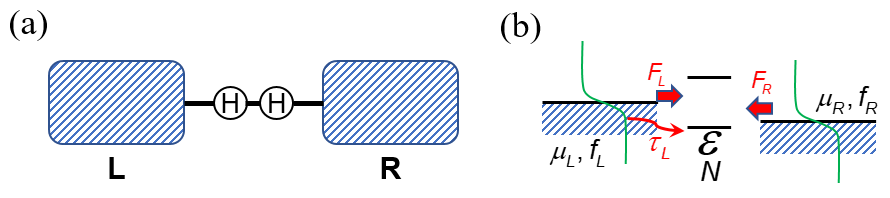
\includegraphics[width=\textwidth]{figures/Fig1_1}
\caption{\small (a) Schematic diagram of the "hydrogen molecule" device with left (L) and right (R) contact. (b) Energy diagram when applying a bias $-eV = \mu_{R}-\mu_{L}$. $F_{L,R}$ and $f_{L,R}$ are the electron flux and Fermi function of the left and right contacts. The green curves indicate the probability distribution of finding an electron (Fermi distribution).}
\end{figure}
We assume that when applying a bias $V$, the electrons can flow through the hydrogen molecule without scattering. Also, the Fermi function (distribution) is not applicable for the hydrogen molecule because the amount of electrons is not sufficient to be statistically meaningful\footnote{Ashley H. Carter, Classical and Statistical Thermodynamics.}. However, the contacts (like electron reservoirs) are assumed to be "large" enough to support the Fermi function. The equation of states (continuity equation) at a given energy $\varepsilon_i$ can be written as 
\begin{equation}
\frac{dN^{\varepsilon_i}}{dt} = F^{\varepsilon_i}_{L} + F^{\varepsilon_i}_{R}
\end{equation} 
where $N^{\epsilon_i}$ is the occupation factor at energy $\epsilon_i$ and the fluxes are 
\begin{equation}
F^{\varepsilon_i}_{L} = \frac{f^{\varepsilon_i}_{L}-N^{\varepsilon_i}}{\tau^{\varepsilon_i}_{L}}
\end{equation}
\begin{equation}
F^{\varepsilon_i}_{R} = \frac{f^{\varepsilon_i}_{R}-N^{\varepsilon_i}}{\tau^{\varepsilon_i}_{R}}
\end{equation} 
Hence, Equation (1.5) becomes\footnote{The superscript $\varepsilon_i$ is omitted for simplicity.} 
\begin{equation}
\frac{dN}{dt} + N \left(\frac{1}{\tau_{L}}+\frac{1}{\tau_{R}}\right) = \frac{f_{L}}{\tau_{L}}+\frac{f_{R}}{\tau_{R}}
\end{equation} 
Now, we define\footnote{The physical meaning will be discussed later.} 
\begin{equation}
\frac{1}{\tau_{L,R}} = \frac{\gamma_{L,R}}{\hbar}
\end{equation} where $\gamma$ has the unit of energy. Thus, we get 
\begin{equation}
\hbar \frac{dN}{dt} + N \left(\gamma_{L}+\gamma_{R}\right) = \gamma_{L} f_{L} + \gamma_{R} f_{R}
\end{equation} 
At steady state, we have 
\begin{equation}
N = \frac{\gamma_{L} f_{L} + \gamma_{R} f_{R}}{\gamma_{L}+\gamma_{R}}
\end{equation} 
Therefore, the current at energy $\varepsilon_i$ can be expressed as 
\begin{align}
I^{\varepsilon_i}&= e F^{\varepsilon_i}_{L} = e \frac{f^{\varepsilon_i}_{L}-N^{\varepsilon_i}}{\tau^{\varepsilon_i}_{L}}\nonumber\\
&=\frac{e}{\hbar} \gamma^{\varepsilon_i}_{L} \left(f^{\varepsilon_i}_{L}-\frac{\gamma^{\varepsilon_i}_{L} f^{\varepsilon_i}_{L} + \gamma^{\varepsilon_i}_{R} f^{\varepsilon_i}_{R}}{\gamma^{\varepsilon_i}_{L}+\gamma^{\varepsilon_i}_{R}}\right)\nonumber\\
&=\frac{e}{\hbar}\frac{\gamma^{\varepsilon_i}_{L}\gamma^{\varepsilon_i}_{R}}{\gamma^{\varepsilon_i}_{L}+\gamma^{\varepsilon_i}_{R}}\left(f^{\varepsilon_i}_{L}-f^{\varepsilon_i}_{R}\right)
\end{align} 
From Equation (1.12), one may directly observe that the current only depends on the properties of the contacts. Now if there are multiple energy levels, the current becomes
\begin{equation}
I = \sum_{\varepsilon_i} I^{\varepsilon_i} \times 2 = \sum_{\varepsilon_i}{\frac{e}{\hbar}\frac{\gamma^{\varepsilon_i}_{L}\gamma^{\varepsilon_i}_{R}}{\gamma^{\varepsilon_i}_{L}+\gamma^{\varepsilon_i}_{R}}\left(f^{\varepsilon_i}_{L}-f^{\varepsilon_i}_{R}\right)}\times2
\end{equation} 
where 2 is coming from the spin degeneracy. Use the following trick 
\begin{equation}
g\left(\varepsilon_i\right) = \int dE g\left(E\right) \delta\left(E-\varepsilon_i\right)
\end{equation} 
and Equation (1.13) can be rewritten as 
\begin{align}
I&= \int dE \left(\frac{2e}{\hbar}\right)\frac{\gamma^{E}_{L}\gamma^{E}_{R}}{\gamma^{E}_{L}+\gamma^{E}_{R}}\left(f^{E}_{L}-f^{E}_{R}\right)\sum_{\varepsilon_i}{\delta\left(E-\varepsilon_i \right)}\nonumber\\
&= \frac{2e}{\hbar}\int dE D\left(E\right) \frac{\gamma^E_{L}\gamma^E_{R}}{\gamma^E_{L}+\gamma^E_{R}} \left(f^E_{L}-f^E_{R}\right)
\end{align} 
where Equation (1.15) is {\bf Landauer's formula} and $D\left(E\right)$ is the density of states (DOS). 
\begin{equation}
D\left(E\right) = \sum_{\varepsilon_i}{\delta\left(E-\varepsilon_i\right)}
\end{equation} 
The general definition of DOS is the number of states per unit energy, so $D\left(E\right)$ also can be written as 
\begin{equation}
D\left(E\right) = \frac{\partial N^{CS}_{E}}{\partial E} = \lim_{\Delta E\rightarrow 0} \frac{N^{CS}_{E}\left(E+\Delta E\right)-N^{CS}_{E}\left(E\right)}{\Delta E}
\end{equation} 
where $N^{CS}_{E}$ is\footnote{Here is the cumulative sum (CS) of states at and below a given energy $E$.} 
\begin{equation}
N_{E}^{CS} = \sum_{\varepsilon_i}{\theta\left(E-\varepsilon_i\right)}
\end{equation} 
where $\theta\left(E-\varepsilon_i\right)$ is the Heaviside step function with the implicit degeneracy as shown in Fig. 1.2. For example, at energy $\varepsilon_{1}$ there are 5 states [Fig. 1.2(a)]. As it goes from low energy to high energy, the cumulative sum of states increases from 5 to 17 [Fig. 1.2(b)].
\begin{figure}[tbp]
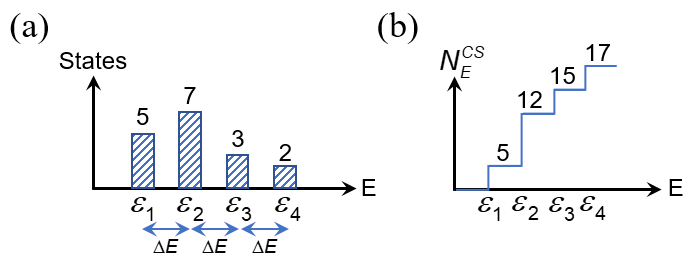
\includegraphics[width=0.7\textwidth]{figures/Fig1_2}
\centering
\caption{\small (a) Number of states distribution. (b) Cumulative sum of states.}
\end{figure} Thus, the Equation (1.17) becomes \begin{equation}
D\left(E\right) = \frac{\partial N^{CS}}{\partial E} = \sum_{\varepsilon_{i}}{\delta\left(E-\varepsilon_{i}\right)}
\end{equation} where $\delta\left(E-\varepsilon_{i}\right)$ is the delta function. After knowing the DOS, we obtain the total occupation factor $N$ 
\begin{align}
N&= \sum_{\varepsilon_{i}}{\frac{\gamma^{\varepsilon_i}_{L} f^{\varepsilon_i}_{L} + \gamma^{\varepsilon_i}_{R} f^{\varepsilon_i}_{R}}{\gamma^{\varepsilon_i}_{L}+\gamma^{\varepsilon_i}_{R}}}\nonumber\\
&= \int dE \frac{\gamma^E_{L} f^E_{L} + \gamma^E_{R} f^E_{R}}{\gamma^E_{L}+\gamma^E_{R}} \sum_{\varepsilon_{i}}{\delta\left(E-\varepsilon_{i}\right)}\nonumber\\
&= \int dE \frac{\gamma^E_{L} f^E_{L} + \gamma^E_{R} f^E_{R}}{\gamma^E_{L}+\gamma^E_{R}}D\left(E\right)
\end{align} 
Equation (1.20) is under the non-equilibrium condition. At the equilibrium condition (applied voltage $V = 0$), the Fermi functions and $\gamma$ of both contacts are the same ($f^E_{L} = f^E_{R} = f^E_{0}, \gamma^E_{L} = \gamma^E_{R}, \forall E$). Thus, the Equation (1.20) can be re-written as 
\begin{equation}
N = \int_{-\infty}^{\infty} D\left(E\right) f_{0}\left(E\right)dE
\end{equation} 
Equation (1.21) is commonly used to calculate the carrier concentration in semiconductors.\\
Now, we would like to figure out the maximum conductance based on Landauer's formula. Two assumptions are made in the following discussion: (1) the applied voltage $V$ is very small and (2) the temperature is fairly low. At small $V$, the Taylor expansion with the first two terms can be applied to the Fermi functions. 
\begin{equation}
    f_{L} = f_{0}\left(E-\mu_{L}\right)
\end{equation} 
\begin{align}
    f_{R}&= f_{0}\left(E-\mu_{R}\right)\nonumber\\
    &= f_{0}\left(E+eV-\mu_{L}\right)\nonumber\\
    &= f_{0}\left(E-\mu_{L}\right)+\left(\frac{\partial f_{0}}{\partial E}\right)eV
\end{align} 
Therefore, the Landauer's formula becomes 
\begin{align}
    I&= \frac{2e}{\hbar}\int dE D\left(E\right) \frac{\gamma^E_{L}\gamma^E_{R}}{\gamma^E_{L}+\gamma^E_{R}} \left(f^E_{L}-f^E_{R}\right)\nonumber\\
    &\approx \frac{2e^{2}}{\hbar}V\int dE D\left(E\right) \frac{\gamma^E_{L}\gamma^E_{R}}{\gamma^E_{L}+\gamma^E_{R}}\left(\frac{-\partial f_{0}}{\partial E}\right)
\end{align} 
Hence, the conductance $G$ is
\begin{equation}
    G = \frac{\partial I}{\partial V} = \frac{2e^{2}}{\hbar}\int dED\left(E\right) \frac{\gamma^E_{L}\gamma^E_{R}}{\gamma^E_{L}+\gamma^E_{R}}\left(\frac{-\partial f_{0}}{\partial E}\right)
\end{equation} 
When the temperature approaches zero, the derivative of the Fermi function with respect to the energy $E$ is like a delta function (see Fig. 1.3) 
\begin{figure}[tbp]
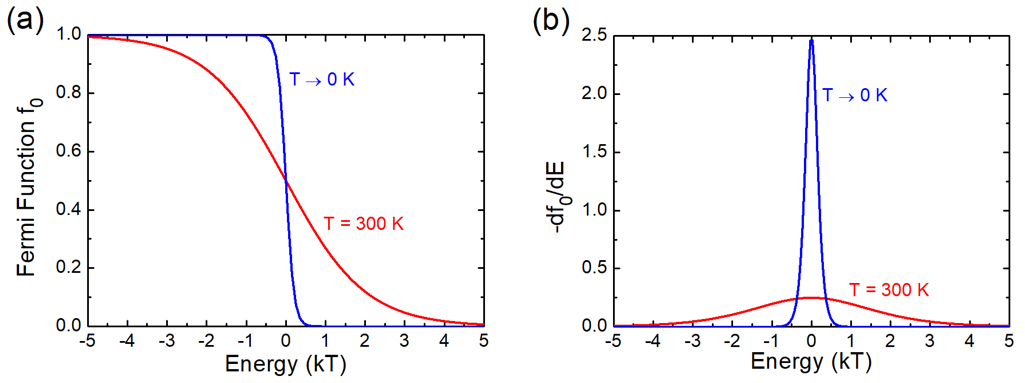
\includegraphics[width=0.9\textwidth]{figures/Fig1_3}
\centering
\caption{\small (a) Fermi functions and (b) their derivative at different temperatures. The Fermi level is located at $E = 0$.}
\end{figure}
\begin{equation}
    \left(\frac{-\partial f_{0}\left(E - \mu_L \right)}{\partial E}\right) \rightarrow \delta\left(E-\mu_{L}\right)
\end{equation} and the conductance $G$ becomes 
\begin{align}
    G& = \frac{2e^{2}}{\hbar}\int dE D\left(E\right) \frac{\gamma^E_{L}\gamma^E_{R}}{\gamma^E_{L}+\gamma^E_{R}}\delta\left(E-\mu_{L}\right)\nonumber\\
    &= \frac{2e^{2}}{\hbar}\left[D\left(E\right)\frac{\gamma^E_{L}\gamma^E_{R}}{\gamma^E_{L}+\gamma^E_{R}}\right]_{E = \mu_L}
\end{align} 
To further examine the Equation (1.27), the concept of "energy broadening" should be introduced.

%%%%%%%%%%%%%%%%%%%%%%%%%%%%%%%%%%%%%%%%%%%%%%%%%
\section{Broadening and Maximum Conductance}
Due to the wave nature of the quantum objects, the uncertainty principle is inherent in the system we discussed. The uncertainty principle states that complementary variables, such as position/momentum and energy/time, cannot be measured simultaneously\footnote{D. J. Griffiths, Introduction to Quantum Mechanics, Chapter 3.}. 
\begin{equation}
    \Delta E \Delta t \geq \frac{\hbar}{2}
\end{equation} 
The $\Delta t$ can be interpreted as the ``lifetime" of electrons, implying that the $\Delta E$ is non-zero, which is called energy ``broadening." This effect has been seen in Equation (1.9) where $\gamma$ is interpreted as the energy broadening. When the atomistic device interacts with a large quantum system (L and R contacts), the energy levels no longer remain discrete but change to a spectrum-like distribution (broadening). However, the shape of the energy broadening is difficult to be experimentally determined, so we utilize the Lorentzian equation\footnote{We would like a function with (1) symmetry and (2) area under the curve $=1$.} to get analytic results \begin{equation}
    \delta\left(E-\varepsilon_{i}\right) \xrightarrow{\text{Broadening}} \frac{1}{2\pi}\frac{\gamma_{L}+\gamma_{R}}{\left(E-\varepsilon_{i}\right)^{2}+\left(\frac{\gamma_{L}+\gamma_{R}}{2}\right)^{2}}
\end{equation} 
For the Lorentzian equation, $\gamma_{L/R}$ are constants and not a function of energy. Then Equation (1.29) gives 
\begin{equation}
    \int_{-\infty}^{\infty} dE \frac{1}{2\pi}\frac{\gamma_{L}+\gamma_{R}}{\left(E-\varepsilon_{i}\right)^{2}+\left(\frac{\gamma_{L}+\gamma_{R}}{2}\right)^{2}} = \frac{\gamma_{L}+\gamma_{R}}{2\pi}\frac{2}{\gamma_{L}+\gamma_{R}}\arctan\left({\frac{E-\varepsilon_{i}}{\frac{\gamma_{L}+\gamma_{R}}{2}}}\right)\bigg|_{-\infty}^{\infty}=1
\end{equation} 
Therefore, the Equation (1.27) can be re-written as 
\begin{align}
    G& = \frac{2e^{2}}{\hbar}\sum_{\varepsilon_{i}}{\delta\left(E-\varepsilon_{i}\right)} \frac{\gamma^E_{L}\gamma^E_{R}}{\gamma^E_{L}+\gamma^E_{R}}\bigg|_{E=\mu_{L}}\nonumber\\
    &\xrightarrow{\text{Broadening}} \frac{2e^{2}}{\hbar}\sum_{\varepsilon_{i}}{\frac{1}{2\pi}\frac{\gamma_{L}+\gamma_{R}}{\left(\mu_{L}-\varepsilon_{i}\right)^{2}+\left(\frac{\gamma_{L}+\gamma_{R}}{2}\right)^{2}}} \frac{\gamma_{L}\gamma_{R}}{\gamma_{L}+\gamma_{R}}\nonumber\\
    &= \frac{2e^{2}}{h}\sum_{\varepsilon_{i}}{\frac{4\gamma_{L}\gamma_{R}}{4\left(\mu_{L}-\varepsilon_{i}\right)^{2}+\left(\gamma_{L}+\gamma_{R}\right)^{2}}}\nonumber\\
    &\xrightarrow[\mu_{L}=\varepsilon_{i}]{maximum} \frac{2e^{2}}{h}{\frac{4\gamma_{L}\gamma_{R}}{\left(\gamma_{L}+\gamma_{R}\right)^{2}}M}
\end{align} 
M is the number of degenerate states at energy $\varepsilon_i$ called the number of modes. From the inequality of arithmetic and geometric means\footnote{$\frac{a+b}{2}\geq\sqrt{ab}\Rightarrow\frac{4ab}{\left(a+b\right)^{2}}\leq1$}, the maximum conductance is \begin{equation}
    G^{max} = \frac{2e^{2}}{h}M
\end{equation} 
Equation (1.32) indicates that the material band structure and dimensionality limit the maximum conductance. This is also why plateaus are observed in the conductance measurement at low temperatures.

%%%%%%%%%%%%%%%%%%%%%%%%%%%%%%%%%%%%%%%%%%%%%%%
\section{Electrostatics}
In the previous sections, the device with two terminals is discussed. Now, let's consider a three-terminal device (like MOSFET) with an insulator layer and a gate contact on the top of the channel as shown in Fig. 1.4.
\begin{figure}[tbp]
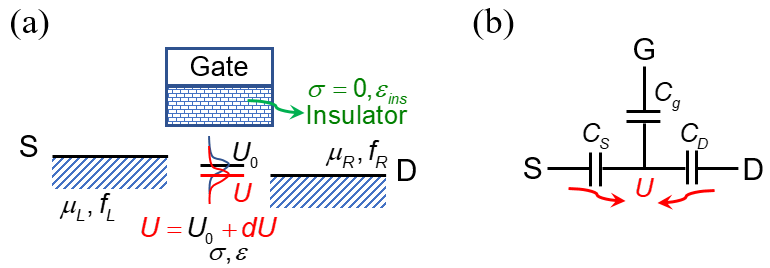
\includegraphics[width=0.8\textwidth]{figures/Fig1_4}
\centering
\caption{\small (a) Schematic diagram of the gated device. The energy level in the channel is broadened due to the current flow. (b) The equivalent circuit of the gated device. $U$ and $U_{0}$ are the energy with and without biases.}
\end{figure} When the gate voltage is applied ($V_{g} \neq 0, V_{S} = V_{D} = 0$), the energy level in the channel is pulled down due to more electrons induced and the change in the electrostatic potential ($\phi$) in the channel can be expressed as 
\begin{equation}
    d\phi = \frac{C_{g}}{C_{g}+C_{S}+C_{D}}dV_{g}
\end{equation}
and the occupation factor with ($N$) and without bias ($N_{0}$)  are \begin{equation}
    N = \int_{-\infty}^{\infty} dE \frac{\gamma_{L} f_{L} + \gamma_{R} f_{R}}{\gamma_{L}+\gamma_{R}}D\left(E-U\right)
\end{equation}
\begin{equation}
    N_{0} = \int_{-\infty}^{\infty} dE \frac{\gamma_{L} f_{L} + \gamma_{R} f_{R}}{\gamma_{L}+\gamma_{R}}D\left(E-U_{0}\right)
\end{equation}
\begin{equation}
    \delta N \equiv N - N_{0}
\end{equation} Similarly, if $V_{S} \neq 0, V_{g} = V_{D} = 0$, the potential change is \begin{equation}
    d\phi = \frac{C_{S}}{C_{g}+C_{S}+C_{D}}dV_{S}
\end{equation} and if $V_{D} \neq 0, V_{g} = V_{S} = 0$, \begin{equation}
    d\phi = \frac{C_{D}}{C_{g}+C_{S}+C_{D}}dV_{D}
\end{equation} Finally, if $V_{g} = V_{S} = V_{D} = 0$, and $Q$ is the amount of charge present in the channel, 
\begin{equation}
    d\phi = \frac{dQ}{C_{g}+C_{S}+C_{D}}
\end{equation} Combining above equations, we obtain \begin{equation}
    d\phi = \alpha_{g} dV_{g} + \alpha_{D} dV_{D} + \alpha_{S} dV_{S} + \frac{dQ}{C_{g}+C_{S}+C_{D}}
\end{equation} where \begin{equation}
    \alpha_{g,S,D} = \frac{C_{g,S,D}}{C_{g}+C_{S}+C_{D}}
\end{equation} The Equation (1.40) also can be expressed using energy $U$ (Multiplying $-e$ to the above equation) 
\begin{align}
    dU& = \alpha_{g} U_{g} + \alpha_{D} U_{D} + \alpha_{S} U_{S} - \frac{edQ}{C_{g}+C_{S}+C_{D}}\nonumber\\
    & = \alpha_{g} U_{g} + \alpha_{D} U_{D} + \alpha_{S} U_{S} - \frac{e^{2}\delta N}{C_{g}+C_{S}+C_{D}}
\end{align} The Equation (1.42) tells us that when increasing the number of electrons (occupation) in the channel, there is an energy penalty that resists the changes. Solving Equation (1.34), (1.35), (1.36), and (1.42) by iterations, the energy $U$ is obtained and the current can be immediately calculated using Landauer's formula \begin{equation}
    I = \frac{2e}{\hbar}\int dE D\left(E-U\right) \frac{\gamma_{L}\gamma_{R}}{\gamma_{L}+\gamma_{R}} \left(f_{L}-f_{R}\right)
\end{equation} where we define 
\begin{equation}
    D\left(E-U\right) \frac{\gamma_{L}\gamma_{R}}{\gamma_{L}+\gamma_{R}} \equiv T\left(E\right)
\end{equation} is the transmission probability due to scatterings. Assuming the applied drain-to-source voltage ($V$) is small and the energy broadening follows Equation (1.29), we have 
\begin{align}
    I& = \frac{2e}{\hbar}\sum_{\varepsilon_{i}}{\int dE \frac{1}{2\pi}\frac{\gamma_{L}+\gamma_{R}}{\left(E-\varepsilon_{i}\right)^{2}+\left(\frac{\gamma_{L}+\gamma_{R}}{2}\right)^{2}} \frac{\gamma_{L}\gamma_{R}}{\gamma_{L}+\gamma_{R}} \left(\frac{-\partial f_{0}}{\partial E}\right)eV}\nonumber\\
    &= \frac{2e^2}{h}V\sum_{\varepsilon_{i}}{\underbrace{\int dE\times \frac{\gamma_{L}\gamma_{R}}{\left(E-\varepsilon_{i}\right)^{2}+\left(\frac{\gamma_{L}+\gamma_{R}}{2}\right)^{2}} \left(\frac{-\partial f_{0}}{\partial E}\right)}_{\equiv \overline{T}_{}\varepsilon_{i}}}\nonumber\\
    &= \frac{2e^{2}}{h}V\overline{M}\cdot\overline{T}_{\varepsilon_{i}}
\end{align} where $\overline{M}$ is the average number of modes around the Fermi energy. The resistance is \begin{equation}
    R = \frac{\partial V}{\partial I} = \frac{h}{2e^{2}\overline{M}}\cdot\frac{1}{\overline{T}_{\varepsilon_{i}}}
\end{equation} 

Thus, the question is: how to determine $\overline{T}_{\varepsilon_{i}}$? Let's consider two scattering events in the channel as shown in Fig. 1.5.
\begin{figure}[tbp]
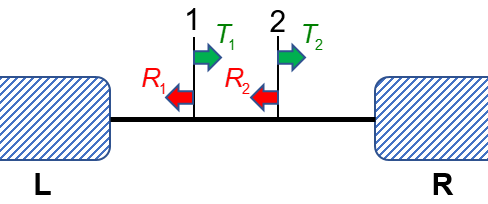
\includegraphics[width=0.5\textwidth]{figures/Fig1_5}
\centering
\caption{\small Two scattering events 1 and 2 with reflection $R$ and transmission $T$.}
\end{figure} The total transmission $T$ is \begin{align}
    T& = T_{1}T_{2} + T_{1}R_{2}R_{1}T_{2} + T_{1}T_{2}\left(R_{2}R_{1}\right)^{2} + \cdots\nonumber\\
    &= T_{1}T_{2}\left(1 + R_{1}R_{2} + \left(R_{2}R_{1}\right)^{2} + \cdots\right)\nonumber\\
    &= \frac{T_{1}T_{2}}{1-R_{1}R_{2}} = \frac{T_{1}T_{2}}{1-\left(1-T_{1}\right)\left(1-T_{2}\right)} = \frac{T_{1}T_{2}}{T_{1}+T_{2}-T_{1}T_{2}}\nonumber
\end{align} \begin{align}
    \Rightarrow \frac{1}{T}& = \frac{T_{1}+T_{2}-T_{1}T_{2}}{T_{1}T_{2}}\nonumber
\end{align} \begin{align}
    \Rightarrow \frac{1-T}{T}& = \frac{T_{1}+T_{2}-2T_{1}T_{2}}{T_{1}T_{2}}\nonumber\\
    &= \frac{1-T_{1}}{T_{1}} + \frac{1-T_{2}}{T_{2}}
\end{align} Therefore, if there are $N$ scattering events and the channel length is $L$, the total transmission $T$ probability is \begin{equation}
    \frac{1-T}{T} = \sum_{i}^{N}{\frac{1-T_{i}}{T_{i}}}
\end{equation} Assume the transmission probability of each scattering event is identical ($T_{1} = T_{2} = \cdots = T_{k}$), we have \begin{equation}
    \frac{1-T}{T} = \frac{N\left(1-T_{k}\right)}{T_{k}}\nonumber
\end{equation} \begin{equation}
    \Rightarrow \frac{1}{T} = \frac{N\left(1-T_{k}\right)+T_{k}}{T_{k}}
\end{equation} Define \begin{equation}
    \nu \equiv \frac{N}{L}
\end{equation} The Equation (1.49) becomes \begin{align}
    \frac{1}{T}&= \frac{\nu L \left(1-T_{k}\right)+T_{k}}{T_{k}}\nonumber\\
    &= \frac{L+\frac{T_{k}}{\nu\left(1-T_{k}\right)}}{\frac{T_{k}}{\nu\left(1-T_{k}\right)}}\nonumber\\
    &= \frac{L+T_{k}\lambda}{T_{k}\lambda}\nonumber\\
    &= \frac{L+\lambda'}{\lambda'}
\end{align} where \begin{equation}
    \nu\left(1-T_{k}\right) \equiv \frac{1}{\lambda}
\end{equation} and \begin{equation}
    \lambda' \equiv T_{k}\lambda
\end{equation} Here, $\lambda$ and $\lambda'$ are the mean free path, and $\lambda \approx \lambda'$\footnote{For one-dimensional channel, $T_{k} \approx 1$. Otherwise, the electrons will be localized.}. Therefore, the resistance becomes \begin{equation}
    R = \frac{\partial V}{\partial I} = \frac{h}{2e^{2}\overline{M}}\cdot\left(1+\frac{L}{\lambda'}\right)
\end{equation}
\begin{figure}[tbp]
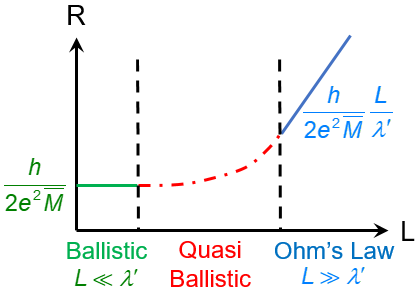
\includegraphics[width=0.4\textwidth]{figures/Fig1_6}
\centering
\caption{\small Resistance $R$ versus channel length $L$ with three regions: ballistic, quasi-ballistic, and Ohm's law.}
\end{figure} Fig. 1.6 shows the resistance versus the channel length. At $L \gg \lambda'$ limit, the Equation (1.54) reduces back to Ohm's law as mentioned in Section 1.1. At $L \ll \lambda'$ limit (ballistic limit without any scattering), the resistance is governed by $\frac{h}{2e^{2}\overline{M}}$ which sets the upper limit of the conductivity. Between above two regions, it's quasi-ballistic region where is the main focus of the discussion in next few chapters.


\chapter{Density of States}
\section{Schrodinger Equation}
Although the classical physics was well developed in 1900s, the black body radiation implicitly indicated that something is missing in the classical physics. From classical physics, the more heat putting in an object would increase the kinetic energy of the object, and thus the energy of the emitted radiation should increase with the frequency which is known as "ultraviolet catastrophe." However, this contradicted with the experimental results that the radiation intensity tends to be zero at short wavelength (higher frequency) regime. To explain this black body radiation, the (implicit) emitted energy quantization and concept of photon (particle of light) were proposed by Planck in 1900\footnote{Einstein explicitly assumed that the electromagnetic radiation is quantized in 1905.}. After that, physicists gradually noticed that every object exhibits both wave-particle duality and the energy states of a system are quantized. Finally, in 1925 Schrodinger wrote down an equation analogous to a wave equation: Schrodinger equation \begin{equation}
    i\hbar\frac{\partial \Psi}{\partial t} = -\frac{\hbar^{2}}{2m_{0}}\frac{\partial^{2}}{\partial x^{2}}\Psi + V\Psi
\end{equation} where $\Psi$ is the wavefunction of a particle, $m_{0}$ is the rest mass of the particle, and $V$ is the potential energy experienced by a particle.
\subsection{Time-Independent Schrodinger Equation}
The time independent Schrodinger equation\footnote{D. J. Griffiths, Introduction to Quantum Mechanics, Chapter 2.} predicts that the wavefunctions are able to form the standing waves which is called stationary states (also called "orbitals," such as atomic orbitals and molecular orbitals). In stationary states, the wavefunction can be divided into two parts using separation of variation method: \begin{equation}
    \Psi = \psi\left(x\right) \varphi\left(t\right)
\end{equation} where $\psi$ is a function of $x$ alone, and $\varphi$ is a function of $t$ alone. There, we can rewrite Equation (2.1) \begin{equation}
    i\hbar\psi\frac{\partial \varphi}{\partial t} = -\frac{\hbar^{2}}{2m_{0}}\frac{\partial^{2}\psi}{\partial x^{2}}\varphi + V\psi\varphi
\end{equation} Dividing through by $\psi\varphi$: \begin{equation}
    i\hbar\frac{1}{\varphi}\frac{\partial \varphi}{\partial t} = -\frac{\hbar^{2}}{2m_{0}}\frac{1}{\psi}\frac{\partial^{2}\psi}{\partial x^{2}} + V
\end{equation} Now, the left side and the right side are functions of $t$ and $x$, respectively\footnote{Here, $V$ is only a function of $x$.}. Thus, both sides are equqal to a constant $E$. Then \begin{equation}
    i\hbar\frac{1}{\varphi}\frac{\partial \varphi}{\partial t} = E
\end{equation} and \begin{equation}
    -\frac{\hbar^{2}}{2m_{0}}\frac{1}{\psi}\frac{\partial^{2}\psi}{\partial x^{2}} + V = E
\end{equation} The general solution of Equation (2.5) is \begin{equation}
    \varphi\left(t\right) = e^{-iEt/\hbar}
\end{equation} and Equation (2.6) becomes \begin{equation}
    -\frac{\hbar^{2}}{2m_{0}}\frac{\partial^{2}\psi}{\partial x^{2}} + V\psi = E\psi \nonumber
\end{equation} Or \begin{equation}
    \boxed{\left[-\frac{\hbar^{2}}{2m_{0}}\frac{\partial^{2}}{\partial x^{2}} + V\right]\psi = E\psi}
\end{equation} The Equation (2.8) is called the {\bf time-independent Schrodinger equation} and \begin{equation}
    -\frac{\hbar^{2}}{2m_{0}}\frac{\partial^{2}}{\partial x^{2}} + V \equiv H
\end{equation} is called the {\bf Hamiltonian} which is an operator. The Equation (2.8) implicitly states that solving the Schrodinger equation is an eigenvalue problem. The physical meaning of the constant $E$ is actually the energy of the particle. Thus, the energy available in a quantum system can be determined by Equation (2.8). Taking a simplest example of a free electron ($V = 0$), we can immediately solve Schrodinger equation and get \begin{equation}
    \psi = A e^{ikx}
\end{equation} and \begin{equation}
    E = \frac{\hbar^{2}k^{2}}{2m_{0}}
\end{equation} where $k$ is the wavenumber. Note that the Equation (2.10) is a plane wave solution. If we apply the periodic boundary condition, we have \begin{equation}
    \psi\left(x=0\right) = \psi\left(x=L\right)\nonumber
\end{equation} \begin{equation}
    1 = e^{ikL} \Rightarrow kL=2\pi n \Rightarrow k = \frac{2\pi}{L}n
\end{equation} and \begin{equation}
    E = \frac{\hbar^{2}}{2m_{0}}\frac{4\pi^{2}}{L^{2}}n^{2}
\end{equation} where $n$ is an integer. Thus, for an one-dimensional free electron, the density of states is \begin{align}
    D\left(E\right)&= \sum_{n}{\delta\left(E-E_{n}\right)} = \sum_{n}{\delta\left(E-\frac{\hbar^{2}}{2m_{0}}\frac{4\pi^{2}}{L^{2}}n^{2}\right)}\nonumber\\
    & = \int_{-\infty}^{\infty}\frac{dk}{\Delta k}\delta\left(E-\frac{\hbar^{2}k^{2}}{2m_{0}}\right),\quad\frac{\hbar^{2}k^{2}}{2m_{0}}\equiv z,\quad \Delta k = \frac{2\pi}{L} \nonumber\\
    & = \frac{Lm_{0}}{\pi\hbar}\frac{1}{\sqrt{2m_{0}}}\int_{0}^{\infty}dz\frac{1}{\sqrt{z}}\delta\left(E-z\right) \nonumber\\
    & = \frac{Lm_{0}}{\pi\hbar}\frac{1}{\sqrt{2m_{0}}}\frac{1}{\sqrt{E}}
\end{align} Note that the electron has up- and down-spin degeneracy, so the total DOS (per unit length per unit energy) is \begin{equation}
    \boxed{\frac{D\left(E\right)}{L} \equiv D\left(E\right) = \frac{2m_{0}}{\pi\hbar}\frac{1}{\sqrt{2m_{0}}}\frac{1}{\sqrt{E}}}
\end{equation}
\subsection{Formalism in Quantum Mechanics}
The formalism in quantum mechanics is somehow different from the classical physics. There are two important constructs: wavefunctions and operators, which represent the state of a system and observables. In mathematical language (linear algebra), the wavefunctions are vectors and, the operators are the linear transformations. A vector in an $N$-dimensional space can be expressed using a specified orthogonal basis \begin{equation}
    \big|\psi\big>\rightarrow\vec{\psi}=
    \left[
    \begin{matrix}
    \phi_{1} \\
    \phi_{2} \\
    \vdots \\
    \phi_{N} \\
    \end{matrix}
    \right]
\end{equation} and \begin{equation}
    \big<\psi\big|\rightarrow\vec{\psi}^{\dagger}=
    \left[
    \begin{matrix}
    \phi_{1}^{*} & \phi_{2}^{*} & \ldots & \phi_{N}^{*}
    \end{matrix}
    \right]
\end{equation} The Equations (2.16) and (2.17) are the ket and bra, which form the {\bf{Dirac notation}}. In general, the solution of Schrodinger equation is \begin{equation}
    \big|\psi\big>=\sum_{j}^{N}{c_{j}\big|\phi_{j}\big>}
\end{equation} and $\phi_{j}$'s form a set of orthogonal basis in $N$-dimensional {\bf Hilbert space} obeying \begin{equation}
    \int_{-\infty}^{\infty}\phi_{i}^{*}\left(x\right)\phi_{j}\left(x\right)dx =
    \begin{cases}
    1 & \text{if }i = j \\
    0 & \text{if }i \neq j
    \end{cases}
\end{equation} where $\phi_{i}^{*}$ is the complex conjugate of $\phi_{i}$ and the Equation (2.19) is the inner product of two bases. The coefficients $c_{j}$'s can be obtained by \begin{equation}
    \boxed{\big<\phi_{k}\big|\psi\big> = \int_{-\infty}^{\infty}\phi_{k}^{*}\left[c_{1}\phi_{1}+c_{2}\phi_{2}+\ldots+c_{k}\phi_{k}+\ldots\right]dx = c_{k}}
\end{equation} Using Dirac notation to rewrite Schrodinger equation, we have\footnote{The bold font represents an operator here and later on. For example, the Hamiltonian is an operator and the energy $E$ is a scalar.} \begin{equation}
    E\big|\psi\big> = \vec{H}\big|\psi\big>
\end{equation} If multiplying $\big<\phi_{k}\big|$ to the Equation (2.21), \begin{equation}
    \sum_{j}Ec_{j}\big<\phi_{k}\big|\phi_{j}\big>=\sum_{j}\big<\phi_{k}\big|\vec{H}c_{j}\big|\phi_{j}\big> \nonumber
\end{equation} \begin{equation}
    \Rightarrow Ec_{k} = \sum_{j}{\big<\phi_{k}\big|\vec{H}\big|\phi_{j}\big>c_{j}} = \sum_{j}{H_{k,j}c_{j}}
\end{equation} where \begin{equation}
    H_{k,j} \equiv \big<\phi_{k}\big|\vec{H}\big|\phi_{j}\big>
\end{equation} Thus, \begin{equation}
    E \left[
    \begin{matrix}
    c_{1} \\
    c_{2} \\
    \vdots \\
    c_{N} \\
    \end{matrix}
    \right] = \left[
    \begin{matrix}
    H_{11}c_{1}+H_{12}c_{2}+\ldots \\
    H_{21}c_{1}+H_{22}c_{2}+\ldots \\
    \vdots \\
    \end{matrix}
    \right] = \vec{H}\left[c\right] \nonumber
\end{equation} \begin{equation}
    \Rightarrow\boxed{E\left[c\right]=\vec{H}\left[c\right]}
\end{equation} The Equation (2.24) explicitly indicates that solving the Schrodinger equation is mathematically an eigenvalue problem, where $\left[c\right]$ is the eigenvectors with the corresponding eigenvalues $E$.
\subsection{Basis Transformation}
As seen in Equation (2.18), there are multiple choices of the set of basis. The question is: how can we change the basis and what are the mathematical and physical meanings of such transformation? Let's consider \begin{equation}
    \big|\psi\big>=\sum_{j}{c_{j}\big|\phi_{j}\big>}=\sum_{k}{d_{k}\big|u_{k}\big>}
\end{equation} \begin{equation}
    \Rightarrow d_{i} = \big<u_{i}\big|\psi\big> = \sum_{j}{\big<u_{i}\big|\phi_{j}\big>c_{j}} \equiv \sum_{j}{M_{ij}c_{j}}
\end{equation} \begin{equation}
    \Rightarrow \left[\begin{matrix}
    d_{1} \\
    d_{2} \\
    \vdots \\
    \end{matrix}
    \right] = \left[M\right]\left[\begin{matrix}
    c_{1} \\
    c_{2} \\
    \vdots \\
    \end{matrix}
    \right]
\end{equation} where $\vec{M}$ is the rotation matrix. Mathematically, the Equation (2.27) represents the rotation of a vector: \begin{equation}
    \vec{A}\big|x\big> = \big|y\big>
\end{equation} and \begin{equation}
    \big<y\big| = \big<x\big|\vec{A}^{\dagger}
\end{equation} such taht \begin{equation}
    \big<y\big|\vec{A}\big|x\big> = \big<y\big|y\big> \nonumber
\end{equation} \begin{equation}
    \Rightarrow \big<x\big|\vec{A}^{\dagger}\vec{A}\big|x\big> = \big<y\big|y\big> = \big<x\big|x\big> = 1
\end{equation} Therefore, \begin{equation}
    \vec{A}^{\dagger}\vec{A} = \vec{I}
\end{equation} where $\vec{I}$ is the identity matrix and the Equation (2.31) is called unitary transformation. Now if we have a two-dimensional vector \begin{equation}
    \big|r\big> = a\big|x\big> + b\big|y\big>
\end{equation} where \begin{equation}
    a = \big<x\big|r\big> \quad \text{and} \quad b = \big<y\big|r\big> \nonumber
\end{equation} then \begin{align}
    \big|r\big>& = \big|x\big>a + \big|y\big>b = \big|x\big>\big<x\big|r\big> + \big|y\big>\big<y\big|r\big>\nonumber \\
    & = \underbrace{\left(\big|x\big>\big<x\big| + \big|y\big>\big<y\big|\right)}_{=1}\big|r\big>
\end{align} More generally, \begin{equation}
    \sum_{i}{\big|\phi_{i}\big>\big<\phi_{i}\big|} = 1
\end{equation} The Equation (2.34) is called the identity operator. By using the identity operator, we obtain the new Hamiltonian in a new set of basis. \begin{align}
    H_{kj}& = \big<u_{k}\big|\vec{H}\big|u_{l}\big>\nonumber\\
    & = \sum_{i,j}{\big<u_{k}\big|\phi_{i}\big>\big<\phi_{i}\big|\vec{H}\big|\phi_{j}\big>\big<\phi_{j}\big|u_{l}\big>} \nonumber\\
    & = \sum_{i,j}{M_{ki}H_{ij}M_{jl}} \nonumber
\end{align} \begin{equation}
    \Rightarrow \vec{M}^{\dagger}\vec{H}^{\text{old}}\vec{M} = \vec{H}^{\text{new}}
\end{equation} As mentioned earlier, solving the Schrodinger equation is a eigenvalue problem. Thus, the property of the Hamiltonian should be properly explored. Suppose we have the following eigenvalue problem \begin{equation}
    \vec{A}\big|x\big> = \lambda\big|x\big> \quad \text{and} \quad \big<x\big|\vec{A}^{\dagger} = \lambda^{\dagger}\big<x\big|
\end{equation} By multiplying $\big<x\big|$ and $\big|x\big>$ from the left and right sides respectively to the Equation (2.36), we have \begin{equation}
    \big<x\big|\vec{A}\big|x\big> = \lambda \quad \text{and} \quad \big<x\big|\vec{A}^{\dagger}\big|x\big> = \lambda^{\dagger}
\end{equation} then \begin{equation}
    \big<x\big|\vec{A}\big|x\big> - \big<x\big|\vec{A}^{\dagger}\big|x\big> = \big<x\big|\vec{A}-\vec{A}^{\dagger}\big|x\big> = \lambda - \lambda^{\dagger} = 0 \quad \text{if} \quad \lambda \in \Re \nonumber
\end{equation} \begin{equation}
    \Rightarrow \vec{A} = \vec{A}^{\dagger}
\end{equation} where $\vec{A}$ is called the {\bf Hermition Matrix}. Because the energy $E$ is real, {\bf the Hamiltonian is also a Hermition matrix}. From Copenhagen interpretation of quantum mechanics, the square of the coefficient $c_{i}$ is the probability having the $i$th state and the total probability of all possible outcomes has to be one \begin{align}
    \big<\psi\big|\psi\big>& = \sum_{ij}{c_{i}^{*}\big<\phi_{i}\big|c_{j}\big|\phi_{j}\big>}\nonumber\\
    & = \sum_{ij}{c_{i}^{*}c_{j}\big<\phi_{i}\big|\phi_{j}\big>} = \sum_{i}{\big|c_{i}\big|^{2}}\nonumber\\
    & = \text{Trace}\left[\begin{matrix}
    \big|c_{1}\big|^{2} & 0 & \ldots \\
    0 & \big|c_{2}\big|^{2} & \ldots \\
    \vdots & \vdots & \ddots
    \end{matrix}
    \right] = 1
\end{align} where each element on the digonal of the matrix is the probability at such state. The momentum operator $\vec{p}$ is\footnote{D. J. Griffiths, Introduction to Quantum Mechanics, Chapter 1.} \begin{equation}
    \vec{p} = -i\hbar\frac{\partial}{\partial x}
\end{equation} Thus, the expectation value of the momentum is\footnote{$\big<x\big|\vec{p}\big|x'\big> = -i\hbar\delta'\left(x-x'\right)$. See R. Shankar, Principles of Quantum Mechanics, second edition, page 64-64.} \begin{align}
    \big<\vec{p}\big>& = \big<\psi\big|\vec{p}\big|\psi\big> = \sum_{ij}{c_{i}^{*}c_{j}\underbrace{\big<\phi_{i}\big|\vec{p}\big|\phi_{j}\big>}_{= \delta_{ij}p_{ij}}} \nonumber\\
    & = \text{Trace}\left(\rho^{\text{eigenbasis}}p^{eigenbasis}\right)
\end{align} where $\rho^{\text{eigenbasis}}$ is the eigenvalue of the density matrix\footnote{It can be interpreted as the probability of having electrons in a given state.}, which is more generally defined as \begin{equation}
    \rho = \sum_{i}{\rho_{i}\big|\phi_{i}\big>\big<\phi_{i}\big|}
\end{equation} where \begin{equation}
    \rho_{i} = \frac{n_{i}}{N} = \big|c_{i}\big|^{2} = \big|\phi_{i}\big>\big<\phi_{i}\big| \quad \text{and} \quad \sum_{i}{\rho_{i}} = 1
\end{equation} $n_{i}$ is the number of particles in the $i$th state and $N$ is the total number of particles in a system. Check consistency of density matrix: \begin{equation}
    n = \int_{-\infty}^{\infty}\frac{\gamma_{1}f_{1}+\gamma_{2}f_{2}}{\gamma_{1}+\gamma_{2}}D\left(E\right)dE
\end{equation} Assume $\gamma_{1} = \gamma_{2}$ and $f_{1} = f_{2} = f_{0}\left(E-\mu\right)$, we have\footnote{There is a confusion here. The unit of the density of states here is {\bf per unit energy}. However, in many semiconductor textbooks, the density of states is in unit of {\bf per unit volume (or area or length) per unit energy}. Thus, $n$ here is the total number of electrons (carriers) instead of density.} \begin{align}
    n& = \int_{-\infty}^{\infty}f_{0}\left(E-\mu\right)D\left(E\right)dE\nonumber\\
    & = \sum_{\varepsilon_{i}}{\int_{-\infty}^{\infty}f_{0}\left(E-\mu\right)\delta\left(E-\varepsilon_{i}\right)dE}\nonumber\\
    & = \sum_{\varepsilon_{i}}{f_{0}\left(E-\mu\right)} = \sum_{i}{n_{i}} = N\big<\psi\big|\psi\big> = N
\end{align}
\section{Bloch's Theorem}
If we want to describe the electron wavefunction in a solid, we need to consider the potential $V$ experienced by the electrons. Let's consider an one-dimensional lattice as shown in Fig. 2.1.
\begin{figure}[tbp]
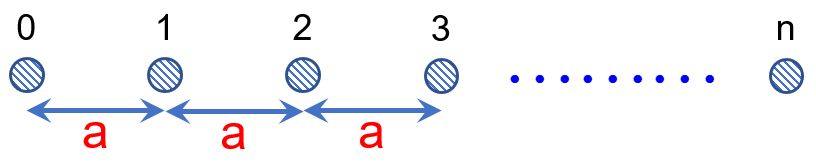
\includegraphics[width=0.7\textwidth]{figures/Fig2_1}
\centering
\caption{\small An one-dimensional lattice with lattice constant of $a$.}
\end{figure} Because there is no way to distinguish the electron wavefunction at each site, the Schrodinger equations of electrons at each site can be written as \begin{equation}
    H\big|\psi\left(\overset{\rightharpoonup}{r}+\overset{\rightharpoonup}{a}\right)\big> = E\big|\psi\left(\overset{\rightharpoonup}{r}+\overset{\rightharpoonup}{a}\right)\big>
\end{equation} \begin{equation}
    H\big|\psi\left(\overset{\rightharpoonup}{r}+2\overset{\rightharpoonup}{a}\right)\big> = E\big|\psi\left(\overset{\rightharpoonup}{r}+2\overset{\rightharpoonup}{a}\right)\big>
\end{equation} and so on. However, above equations imply infinite degeneracy in a solid which is not physical. Therefore, between each wavefunction there should be a scalar multiplier. In other words, \begin{equation}
    \big|\psi\left(\overset{\rightharpoonup}{r}+2\overset{\rightharpoonup}{a}\right)\big> = A\big|\psi\left(\overset{\rightharpoonup}{r}+\overset{\rightharpoonup}{a}\right)\big>
\end{equation} where $A$ is a scalar. Note that \begin{equation}
    \big<\psi\left(\overset{\rightharpoonup}{r}+2\overset{\rightharpoonup}{a}\right)\big|\psi\left(\overset{\rightharpoonup}{r}+2\overset{\rightharpoonup}{a}\right)\big> = A^{*}A\big<\psi\left(\overset{\rightharpoonup}{r}+\overset{\rightharpoonup}{a}\right)\big|\psi\left(\overset{\rightharpoonup}{r}+\overset{\rightharpoonup}{a}\right)\big>\nonumber
\end{equation} \begin{equation}
    \Rightarrow \big|A\big|^{2} = 1 \nonumber \Rightarrow A = e^{i\phi}
\end{equation} Thus, \begin{equation}
    \big|\psi\left(\overset{\rightharpoonup}{r}+n\overset{\rightharpoonup}{a}\right)\big> = e^{in\phi}\big|\psi\left(\overset{\rightharpoonup}{r}\right)\big> \nonumber
\end{equation} or \begin{equation}
    \boxed{\big|\psi\left(\overset{\rightharpoonup}{r}+\overset{\rightharpoonup}{L}\right)\big> = e^{i\overset{\rightharpoonup}{k}\cdot\overset{\rightharpoonup}{L}}\big|\psi\left(\overset{\rightharpoonup}{r}\right)\big>}
\end{equation} where $L (= na)$ is the length of the one-dimensional lattice and $k\left(=\frac{2\pi}{a}\right)$ is the wave number. The Equation (2.49) is called the {\bf Bloch's Theorem}. In general, the Equation (2.49) can be further expressed, for example, in three-dimensional lattice, and the relation between the wave number and the lattice size follows the Fourier transformation. \begin{equation}
    u\left(\overset{\rightharpoonup}{r}\right) = \sum_{g}{A_{g}e^{i\overset{\rightharpoonup}{g}\cdot\overset{\rightharpoonup}{r}}}
\end{equation} where the space spanned by $\overset{\rightharpoonup}{g}$ is called the {\bf reciprocal space} [see Fig. 2.2(b)], and $\overset{\rightharpoonup}{g}$ in three-dimensional lattice is \begin{align}
    \overset{\rightharpoonup}{g}& = \frac{2\pi}{a}n_{1}\hat{x} + \frac{2\pi}{b}n_{2}\hat{y} + \frac{2\pi}{c}n_{3}\hat{z}\nonumber\\
    & = n_{1}\overset{\rightharpoonup}{b_{1}} + n_{2}\overset{\rightharpoonup}{b_{2}} + n_{2}\overset{\rightharpoonup}{b_{2}}
\end{align} where $a$, $b$, and $c$ are the lattice constant of $x$, $y$, and $z$ directions, $n_{i}$'s are the integers, and $\overset{\rightharpoonup}{b_{i}}$'s are \begin{equation}
    \overset{\rightharpoonup}{b_{1}} \equiv \frac{2\pi}{a}\hat{x} \text{,} \quad \overset{\rightharpoonup}{b_{2}} \equiv \frac{2\pi}{b}\hat{y} \text{,} \quad \text{and} \quad \overset{\rightharpoonup}{b_{3}} \equiv \frac{2\pi}{c}\hat{z}
\end{equation} The Equation (2.52) can be generalized \begin{equation}
    \overset{\rightharpoonup}{b_{1}} = 2\pi\frac{\overset{\rightharpoonup}{a_{2}}\times\overset{\rightharpoonup}{a_{3}}}{\overset{\rightharpoonup}{a_{1}}\cdot\left(\overset{\rightharpoonup}{a_{2}}\times\overset{\rightharpoonup}{a_{3}}\right)}\nonumber
\end{equation} \begin{equation}
    \overset{\rightharpoonup}{b_{2}} = 2\pi\frac{\overset{\rightharpoonup}{a_{3}}\times\overset{\rightharpoonup}{a_{1}}}{\overset{\rightharpoonup}{a_{1}}\cdot\left(\overset{\rightharpoonup}{a_{2}}\times\overset{\rightharpoonup}{a_{3}}\right)}\nonumber
\end{equation} \begin{equation}
    \overset{\rightharpoonup}{b_{3}} = 2\pi\frac{\overset{\rightharpoonup}{a_{1}}\times\overset{\rightharpoonup}{a_{2}}}{\overset{\rightharpoonup}{a_{1}}\cdot\left(\overset{\rightharpoonup}{a_{2}}\times\overset{\rightharpoonup}{a_{3}}\right)}
\end{equation} where $\overset{\rightharpoonup}{a_{i}}$'s and $\overset{\rightharpoonup}{b_{i}}$'s are the basis of the real space and reciprocal space, and the denominator is the volume of the unit cell in the real space. Suppose we have a vector constructed by the basis of the real space \begin{equation}
    \overset{\rightharpoonup}{l} = ma\overset{\rightharpoonup}{a_{1}} + nb\overset{\rightharpoonup}{a_{2}} + oc\overset{\rightharpoonup}{a_{3}}
\end{equation} where $m$, $n$, and $o$ are the integers. Then, \begin{align}
    \overset{\rightharpoonup}{g}\cdot\overset{\rightharpoonup}{l}& = \left(n_{1}\overset{\rightharpoonup}{b_{1}} + n_{2}\overset{\rightharpoonup}{b_{2}} + n_{2}\overset{\rightharpoonup}{b_{2}}\right)\cdot\left(ma\overset{\rightharpoonup}{a_{1}} + nb\overset{\rightharpoonup}{a_{2}} + oc\overset{\rightharpoonup}{a_{3}}\right)\nonumber\\
    & = 2\pi\left(n_{1}m + n_{2}n + n_{3}o\right) \equiv 2\pi N
\end{align} This implies that the wavefunction will repeat after a certain translation. If we define $\overset{\rightharpoonup}{k} = \overset{\rightharpoonup}{k'} + \overset{\rightharpoonup}{g}$, the Equation (2.49) becomes \begin{align}
    \psi\left(\overset{\rightharpoonup}{r}+\overset{\rightharpoonup}{L}\right)& = e^{i\overset{\rightharpoonup}{k}\cdot\overset{\rightharpoonup}{L}}\psi\left(\overset{\rightharpoonup}{r}\right) = e^{i\left(\overset{\rightharpoonup}{k'}+\overset{\rightharpoonup}{g}\right)\cdot\overset{\rightharpoonup}{L}}\psi\left(\overset{\rightharpoonup}{r}\right)\nonumber\\
    & = \underbrace{e^{i(2\pi)N}}_{=1}e^{i\overset{\rightharpoonup}{k'}\cdot\overset{\rightharpoonup}{L}}\psi\left(\overset{\rightharpoonup}{r}\right)
\end{align} Since there is no way to distinguish $k$ and $k'$, the wavefunction will repeat after shift $k$ by $2\pi/a$. Within the region where the wavefunction does not repeat, it is called the {\bf Brillouin zone} as shown in Fig. 2.2(a).
\begin{figure}[tbp]
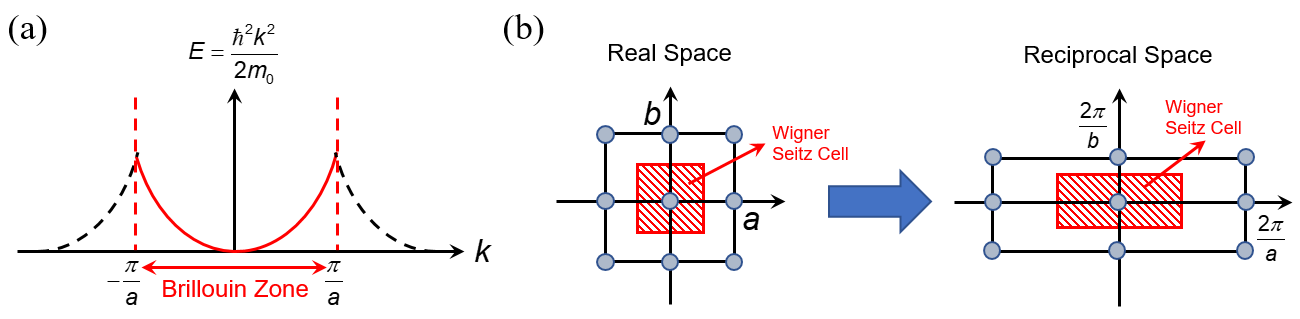
\includegraphics[width=\textwidth]{figures/Fig2_2}
\centering
\caption{\small (a) Dispersion relation ($E-k$) of an one-dimensional lattice. (b) An two-dimensional lattice in real space and reciprocal space.}
\end{figure} A common used method to obtain the Brillouin zone is to draw the {\bf Wigner Seitz cell} which bisects each nearest neighbor as shown in Fig. 2.2(b).
\section{Band Structure}
\subsection{One-Dimensional Monatomic Lattice}
Suppose we have an one-dimensional lattice shown in Fig. 2.1 and assume that the overlap of wavefunctions only presents between nearest neighbor atoms. The elements in Hamiltonian matrix are \begin{equation}
    H_{ii} = \big<\psi_{i}\big|\vec{H}\big|\psi_{i}\big> = t_{0}
\end{equation} \begin{equation}
    H_{i(i\pm 1)} = \big<\psi_{i}\big|\vec{H}\big|\psi_{i(i\pm 1)}\big> = t_{1}
\end{equation} The full matrix looks like \begin{equation}
    \vec{H} = \left[\begin{matrix}
    t_{0} & t_{1} & 0 & 0 & 0 & \ldots \\
    t_{1}^{*} & t_{0} & t_{1} & 0 & 0 & \ldots \\
    0 & t_{1}^{*} & t_{0} & t_{1} & 0 & \ldots \\
    \vdots & \vdots & \vdots & \vdots & \vdots & \ddots
    \end{matrix}
    \right]
\end{equation} The Schrodinger equation becomes\footnote{Each $\psi$ represents the wavefunction of an electron at each lattice site instead of the basis function.} \begin{equation}
    \vec{H}\vec{\psi} = \left[\begin{matrix}
    t_{0} & t_{1} & 0 & 0 & 0 & \ldots \\
    t_{1}^{*} & t_{0} & t_{1} & 0 & 0 & \ldots \\
    0 & t_{1}^{*} & t_{0} & t_{1} & 0 & \ldots \\
    \vdots & \vdots & \vdots & \vdots & \vdots & \ddots
    \end{matrix}
    \right] \left[ \begin{matrix}
    \psi_{1} \\
    \psi_{2} \\
    \psi_{3} \\
    \vdots
    \end{matrix}
    \right] = E\left[ \begin{matrix}
    \psi_{1} \\
    \psi_{2} \\
    \psi_{3} \\
    \vdots
    \end{matrix}
    \right]
\end{equation} At the $n$th row: \begin{equation}
    t_{0}\psi_{n} + t_{1}\psi_{n+1} + t_{1}^{*}\psi_{n-1} = E\psi_{n}
\end{equation} and from Block's theorem \begin{equation}
    \psi_{n} = \psi_{0}e^{ikna}
\end{equation} Thus, we have \begin{equation}
    E = t_{0} + t_{1}e^{ika} + t_{1}^{*}e^{-ika} \xrightarrow{\text{if } t_{1} \text{ is real}} t_{0} + 2t_{1}\cos{ka}
\end{equation} If $ka \ll 1$ and $t_{1} < 0$, the Equation (2.63) can be expanded by using Taylor series. \begin{align}
    E& \simeq t_{0} + 2t_{1}\left[1-\frac{\left(ka\right)^2}{2}+\ldots\right]\nonumber\\
    & = t_{0} + 2t_{1} - \left(t_{1}a^{2}\right)k^{2}\nonumber\\
    & = t_{0} - 2\big|t_{1}\big| + \left(\big|t_{1}\big|a^{2}\right)k^{2}
\end{align} Define the effective mass $m^{*}$ \begin{equation}
    m^{*} = \frac{\hbar^{2}}{2a^{2}\big|t_{1}\big|}
\end{equation} The Equation (2.64) becomes \begin{equation}
    E = E' + \frac{\hbar^{2}}{2m^{*}}k^{2}
\end{equation} where $E'\equiv t_{0}-2\big|t_{1}\big|$. When $\big|t_{1}\big|$ is large, the coupling between the nearest neighbor is strong so that the electron is "de-localized\footnote{The electron can move freely through the lattice sites.}." The effective mass approximation is usually valid for the transport phenomenon in the commonly used semiconductors since the electrons involving the transport are near the bottom of the band (within 1eV). However, when solving the binding strength between the nearest neighbors, this approximation may not be good.
\subsection{One-Dimensional Diatomic Lattice}
The diatomic lattice contains two atoms in a lattice site as shown in Fig. 2.3.
\begin{figure}[tbp]
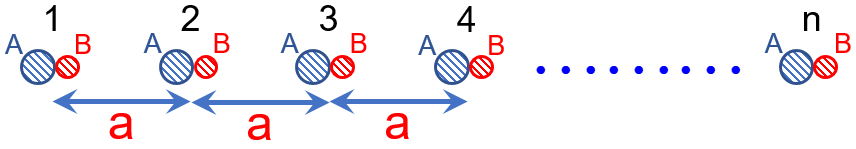
\includegraphics[width=0.7\textwidth]{figures/Fig2_3}
\centering
\caption{\small An one-dimensional diatomic (A and B) lattice with lattice constant of $a$.}
\end{figure} We assume that the wavefunction overlap only happens between the nearest neighbor atoms and atoms on site, i.e., $A_{1}$ and $B_{1}$ or $B_{1}$ and $A_{2}$. Based on this assumption, the Hamiltonian can be expressed as\\
\begin{center}
\begin{tabular}[c]{cc|cc|cc|cc|c}
     &   & 1 & 1 & 2 & 2 & 3 & 3 &  \\
     &   & A & B & A & B & A & B &  \\
     \hline
   1 & A & $t_{0}$ & $t_{1}$ & 0 & 0 & 0 & 0 & \ldots \\
   1 & B & $t_{1}^{*}$ & $t_{0}$ & $t_{2}$ & 0 & 0 & 0 & \ldots \\
     \hline
   2 & A & 0 & $t_{2}^{*}$ & $t_{0}$ & $t_{1}$ & 0 & 0 & \ldots \\
   2 & B & 0 & 0 & $t_{1}^{*}$ & $t_{0}$ & $t_{2}$ & 0 & \ldots \\
     \hline
   3 & A & 0 & 0 & 0 & $t_{2}^{*}$ & $t_{0}$ & $t_{1}$ & \ldots \\
   3 & B & 0 & 0 & 0 & 0 & $t_{1}^{*}$ & $t_{0}$ & \ldots \\
     \hline
     & & \vdots & \vdots & \vdots & \vdots & \vdots & \vdots & $\ddots$ \\
\end{tabular}
\end{center}
At the $n$th row\footnote{Each row represents each lattice site.}, the Schrodinger equation gives \begin{equation}
    \left[H\right]_{n,n}\left[\psi_{0}\right]e^{ikna} + \left[H\right]_{n,n+1}\left[\psi_{0}\right]e^{ikna}e^{ika} + \left[H\right]_{n,n-1}\left[\psi_{0}\right]e^{ikna}e^{-ika} = E\left[\psi_{0}\right]e^{ikna}
\end{equation} \begin{equation}
    \Rightarrow \left[\begin{matrix}
    t_{0} & t_{1}+t_{2}e^{ika} \\
    t_{1}^{*}+t_{2}^{*}e^{-ika} & t_{0}
    \end{matrix}
    \right] \left[\begin{matrix}
    \psi_{0A} \\
    \psi_{0B}
    \end{matrix}
    \right] = E\left[\begin{matrix}
    \psi_{0A} \\
    \psi_{0B}
    \end{matrix}
    \right]\nonumber
\end{equation} \begin{equation}
    \Rightarrow E = t_{0} \pm \sqrt{\big|t_{1}\big|^{2}+\big|t_{2}\big|^{2}+2\text{Re}\left(t_{1}t_{2}e^{ika}\right)}
\end{equation} The Equation (2.68) indicates that there are two bands in this system. If considering more interactions between more basis functions, more bands would be obtained. More generally, the Equation (2.67) can be expressed as \begin{equation}
    \sum_{m}{\left[H\right]_{n} + \left[H\right]_{n,m}e^{i\overset{\rightharpoonup}{k}\cdot\left(\overset{\rightharpoonup}{r_{m}}-\overset{\rightharpoonup}{r}\right)}}
\end{equation} where the first and second terms are the Hamiltonian matrix on the lattice site and the Hamiltonian of the overlap between the nearest neighbors respectively, and $m$ represents the nearest neighbor. The first term also can be absorbed into the second term and the Equation (2.69) becomes \begin{equation}
    \boxed{
    \sum_{m}{\left[H\right]_{n,m}e^{i\overset{\rightharpoonup}{k}\cdot\left(\overset{\rightharpoonup}{r_{m}}-\overset{\rightharpoonup}{r}\right)}} \equiv \left[h(\overset{\rightharpoonup}{k})\right]
    }
\end{equation} which is the {\bf Fourier transformation} between the reciprocal and real spaces.
\subsection{Graphene}
Graphene consists of carbon atoms with two-dimensional hexagonal lattice as shown in Fig. 2.4.
\begin{figure}[tbp]
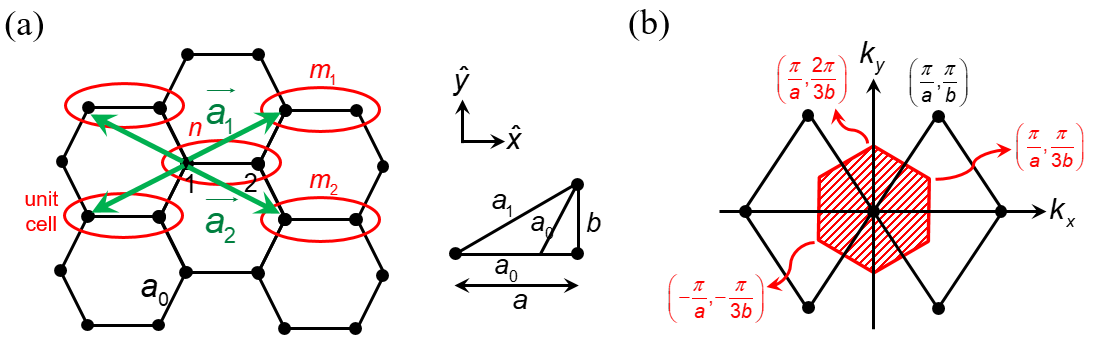
\includegraphics[width=\textwidth]{figures/Fig2_4}
\centering
\caption{\small Graphene in (a) real space (lattice constant is $a_{0}$) and (b) reciprocal space. The green arrows in (a) are the translation vectors ($\overset{\rightharpoonup}{a_{1}}$ and $\overset{\rightharpoonup}{a_{2}}$) and two atoms circled by the red line form the unit cell. The red hexagon is the Wigner Seitz cell (Brillouin zone).}
\end{figure} The coordinate of graphene in real space is defined in Fig. 2.4(a). Thus, the translation vectors in real space are \begin{equation}
    \overset{\rightharpoonup}{a_{1}} = a\hat{x} + b\hat{y}
\end{equation} \begin{equation}
    \overset{\rightharpoonup}{a_{2}} = a\hat{x} - b\hat{y}
\end{equation} \begin{equation}
    \overset{\rightharpoonup}{a_{3}} = \hat{z}
\end{equation} and \begin{equation}
    a = a_{0} + a_{0}\sin{\frac{\pi}{6}} = \frac{3a_{0}}{2}
\end{equation} \begin{equation}
    b = a_{0}\cos{\frac{\pi}{6}} = \frac{\sqrt{3}}{2}a_{0}
\end{equation} Then, the translation vectors in reciprocal space are \begin{equation}
    \overset{\rightharpoonup}{b_{1}} = 2\pi\frac{\overset{\rightharpoonup}{a_{2}}\times\overset{\rightharpoonup}{a_{3}}}{\overset{\rightharpoonup}{a_{1}}\cdot\overset{\rightharpoonup}{a_{2}}\times\overset{\rightharpoonup}{a_{3}}} = \frac{\pi}{a}\hat{x} + \frac{\pi}{b}\hat{y}
\end{equation} \begin{equation}
    \overset{\rightharpoonup}{b_{2}} = \frac{\pi}{a}\hat{x} - \frac{\pi}{b}\hat{y}
\end{equation} Due to weaker coupling of $p_{z}$ orbitals between nearest neighbors than that of $p_{x,y}$, the energy split is smaller (the energy states are closer to the Fermi level) so that the wavefunction overlap of $p_{z}$ orbitals is considered. We also assume that only the wavefunction overlap of the nearest neighbors does matter. Thus, the Hamiltonian matrix of the $n$th unit cell [see Fig. 2.4(a)] can be expressed using the Equation (2.70) \begin{equation}
    \left[H\right]_{n,n} + \left[H\right]_{n,m_{1}}e^{i\overset{\rightharpoonup}{k}\cdot\overset{\rightharpoonup}{a_{1}}} + \left[H\right]_{n,m_{2}}e^{i\overset{\rightharpoonup}{k}\cdot\overset{\rightharpoonup}{a_{2}}} + \left[H\right]_{n,m_{1}}e^{-i\overset{\rightharpoonup}{k}\cdot\overset{\rightharpoonup}{a_{1}}} + \left[H\right]_{n,m_{2}}e^{-i\overset{\rightharpoonup}{k}\cdot\overset{\rightharpoonup}{a_{2}}}
\end{equation} where \begin{equation}
    \left[H\right]_{n,n} = \left[ \begin{matrix}
    t_{0} & t \\
    t & t_{0}
    \end{matrix}
    \right],\quad
    \left[H\right]_{n,m_{1}} = \left[ \begin{matrix}
    0 & 0 \\
    t & 0
    \end{matrix}
    \right],\quad
    \left[H\right]_{n,m_{2}} = \left[ \begin{matrix}
    0 & 0 \\
    t & 0
    \end{matrix}
    \right]
\end{equation} and \begin{equation}
    t_{0} = \big<\psi_{1}\big|\vec{H}\big|\psi_{1}\big>,\quad t = \big<\psi_{1}\big|\vec{H}\big|\psi_{2}\big>,\quad t = t^{*}
\end{equation} Here, $\psi_{1,2}$ are the wavefunctions at the first (left side) and the second (right side) lattice sites in an unit cell. Therefore, the Equation (2.78) is \begin{align}
    \left[h(\overset{\rightharpoonup}{k})\right]& = \left[\begin{matrix}
    t_{0} & t + te^{-i\overset{\rightharpoonup}{k}\cdot\overset{\rightharpoonup}{a_{1}}} + te^{-i\overset{\rightharpoonup}{k}\cdot\overset{\rightharpoonup}{a_{2}}} \\
    t + te^{i\overset{\rightharpoonup}{k}\cdot\overset{\rightharpoonup}{a_{1}}} + te^{i\overset{\rightharpoonup}{k}\cdot\overset{\rightharpoonup}{a_{2}}} & t_{0}
    \end{matrix}
    \right]\equiv \left[\begin{matrix}
    t_{0} & p^{*}(\overset{\rightharpoonup}{k}) \\
    p(\overset{\rightharpoonup}{k}) & t_{0}
    \end{matrix}
    \right]
\end{align} where \begin{align}
    p(\overset{\rightharpoonup}{k})& = t + te^{i\overset{\rightharpoonup}{k}\cdot\overset{\rightharpoonup}{a_{1}}} + te^{i\overset{\rightharpoonup}{k}\cdot\overset{\rightharpoonup}{a_{2}}} = t\left[1+2e^{ik_{x}a}\cos{k_{y}b}\right]
\end{align} The eigenvalue (energy) of the matrix (2.81) is \begin{align}
    E(\overset{\rightharpoonup}{k})& = t_{0} \pm \big|p(\overset{\rightharpoonup}{k})\big|\nonumber\\
    & = t_{0} \pm t\sqrt{1+4\cos^{2}{k_{y}b}+4\cos{k_{x}a}\cos{k_{y}b}}
\end{align} The above equation describes the dispersion relationship ($E$-$k$ diagram) of graphene. Let's now consider $k_{x} = 0$: \begin{equation}
    E = t_{0} \pm t\left(1+2\cos{k_{y}b}\right)
\end{equation} If $t_{0} = 0$ is chosen, the $E$-$k_y$ plot is shown in Fig 2.5.
\begin{figure}[tbp]
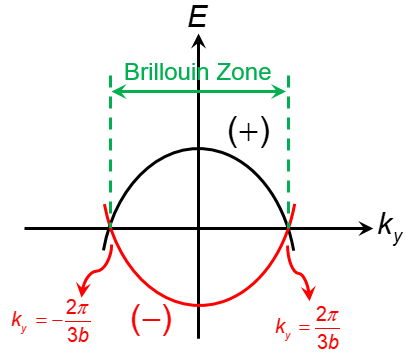
\includegraphics[width=0.4\textwidth]{figures/Fig2_5}
\centering
\caption{\small $E$-$k$ diagram of graphene at $k_{x} = 0$.}
\end{figure} Note that $k_{y} = \pm \frac{2\pi}{3b}$ are the points located at the Brillouin zone boundary as shown in Fig. 2.4(b). These points are called "Dirac points." If $k_{x} \neq 0$, the $E$-$k$ would look like a cone and the $k_{x}$ and $k_{y}$ satisfying $E = 0$ are $\left(\pm\frac{\pi}{a},\pm\frac{\pi}{3b}\right)$ where are at the zone boundary. Because the two bands are crossing at the Dirac points, the graphene behaves like a metal and the number of electrons near the Fermi level ($E_{F} = 0$) is $2\times 2\times 2 = 8$\footnote{2's are coming from two bands, up- and down-spin, and equivalent corner in the Brillouin zone.}. Now, let's consider $E$ near the Dirac point. The Taylor expansion of the Equation (2.83) assuming $t_{0} = 0$ is \begin{align}
    E(\overset{\rightharpoonup}{k})& = \pm \big|p(\overset{\rightharpoonup}{k})\big|\nonumber\\
    & \approx \pm\big|\frac{\partial p}{\partial k_{x}}\big|_{0,\pm \frac{2\pi}{3b}}\left(k_{x}-0\right) + \frac{\partial p}{\partial k_{y}}\big|_{0,\pm \frac{2\pi}{3b}}\left(k_{y}\pm\frac{2\pi}{3b}\right)\big|\nonumber\\
    & = \pm\big|-\frac{3}{2}a_{0}t\left[ik_{x}+\left(k_{y}\mp\frac{2\pi}{3b}\right)\right]\big|\nonumber\\
    & = \pm \frac{3}{2}a_{0}t\sqrt{k_{x}^{2}+\left(k_{y}\mp\frac{2\pi}{3b}\right)^{2}}\\
    & = \pm at\big|k\big| \quad \text{(linear dispersion relationship)}\nonumber
\end{align} which is different from the square dependence of $k$ for the free electron. The definition of the effective mass $m^{*} = \frac{\hbar^{2}}{\frac{\partial^{2} E}{\partial k^{2}}}$ at the Dirac points becomes physically meaningless where defining $p = \hbar k$ would be better. Since $p = 0$ at the Dirac points, there will be no current flow at that points. Around the Dirac point, the electron group velocity is \begin{equation}
    v = \frac{\partial \omega}{\partial k} = \frac{1}{\hbar}\frac{\partial E}{\partial k}=\frac{3}{2}\frac{a_{0}t}{\hbar}=\text{constant}
\end{equation} where $v$ is always written as $v_{F}$ (Fermi velocity). Thus, the E-k relation of graphene also can be written in terms of $v_{F}$ \begin{equation}
    E=\pm\hbar v_{F}\big|k\big|
\end{equation} where the electron behaves like a relativistic particle and cannot be accelerated.
\subsection{Graphene Nanotube}
Since the graphene behaves like a metal, engineering graphene to be semiconductor would be very important. One way to achieve that is to roll it into a tube as shown in Fig. 2.6.
\begin{figure}[tbp]
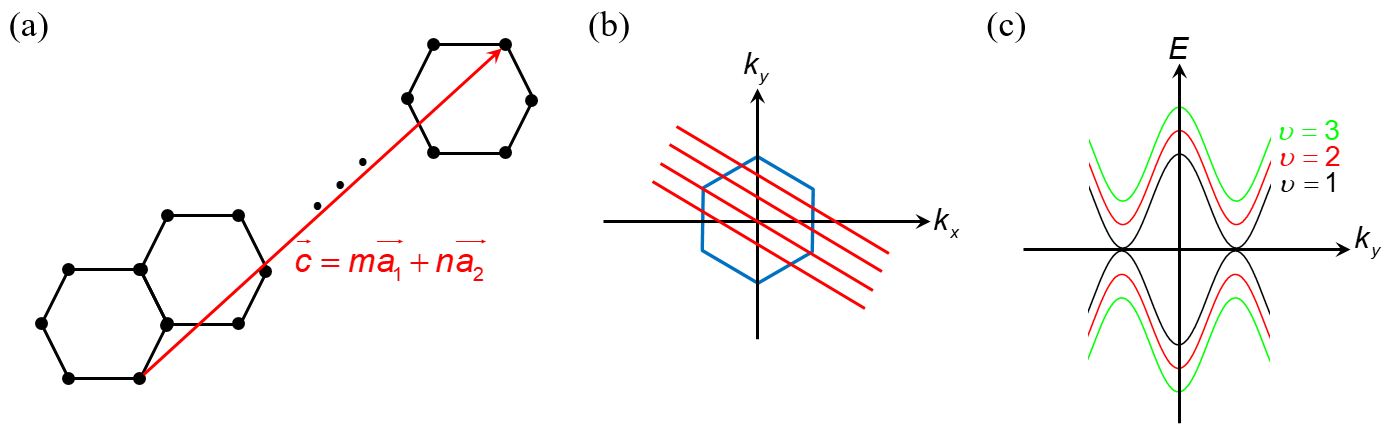
\includegraphics[width=\textwidth]{figures/Fig2_6}
\centering
\caption{\small (a) Graphene with rolling vector $\overset{\rightharpoonup}{c}$. (b) Brillouin zone of graphene and possible solutions (red straight lines) of nanotube. (c) $E-k$ diagram of graphene nanotube, assuming $k_{x}=0$.}
\end{figure} After rolling the graphene, we impose additional restriction to the lattice \begin{equation}
    \overset{\rightharpoonup}{k}\cdot\overset{\rightharpoonup}{c} = 2\pi\nu,\quad \nu\in Z
\end{equation} because the wavefunction will be a periodic function. The Equation (2.88) can be further written as \begin{equation}
    k_{y} = \frac{2\pi}{\left(m-n\right)b}\nu-\frac{\left(m+n\right)a}{\left(m-n\right)b}k_{x}
\end{equation} which represents straight lines shown in Fig. 2.6(b) depending on $\nu$ if $m$ and $n$ are known. Because the corners of the Brillouin zone [see Fig. 2.6(b)] correspond to the Dirac points, the graphene nanotube exhibits the metallic nature if the straight line crosses the corners. Therefore, whether the graphene nanotube behaves like a metal or a semiconductor would depend on how it is rolled (various combinations of $m$ and $n$).
\subsubsection{Armchair Graphene Nanotube}
If the graphene is rolled only in $x$-direction, it's called armchair nanotube as shown in Fig. 2.7.
\begin{figure}[tbp]
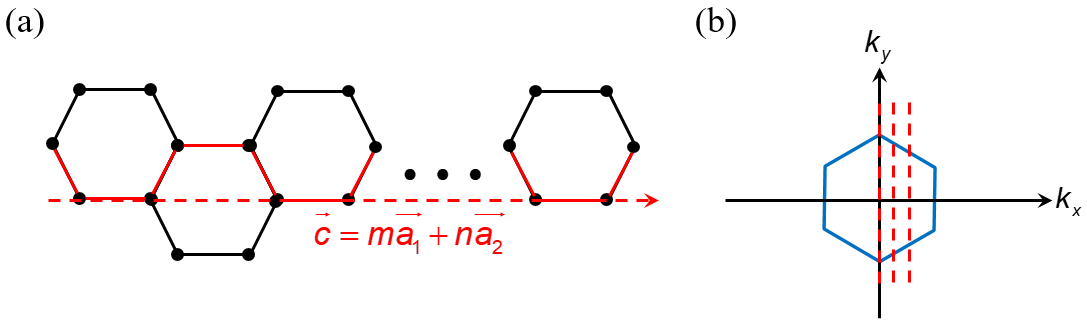
\includegraphics[width=0.9\textwidth]{figures/Fig2_7}
\centering
\caption{\small (a) Illustration of rolling an armchair nanotube. (b) Brillouin zone and possible solutions (straight lines) of armchair nanotube.}
\end{figure} Because now the wavefunction is restricted in $x$-direction, the $k_{y}$ is zero and thus the Equation (2.89) becomes \begin{equation}
    k_{x} = \frac{2\pi}{\left(m+n\right)a}\nu
\end{equation} Since $k_{x} = 0$ is a valid solution, the armchair nanotube is always metallic.
\subsubsection{Zigzag Graphene Nanotube}
If the graphene is rolled only in $y$-direction, it's called zigzag nanotube as shown in Fig. 2.8.
\begin{figure}[tbp]
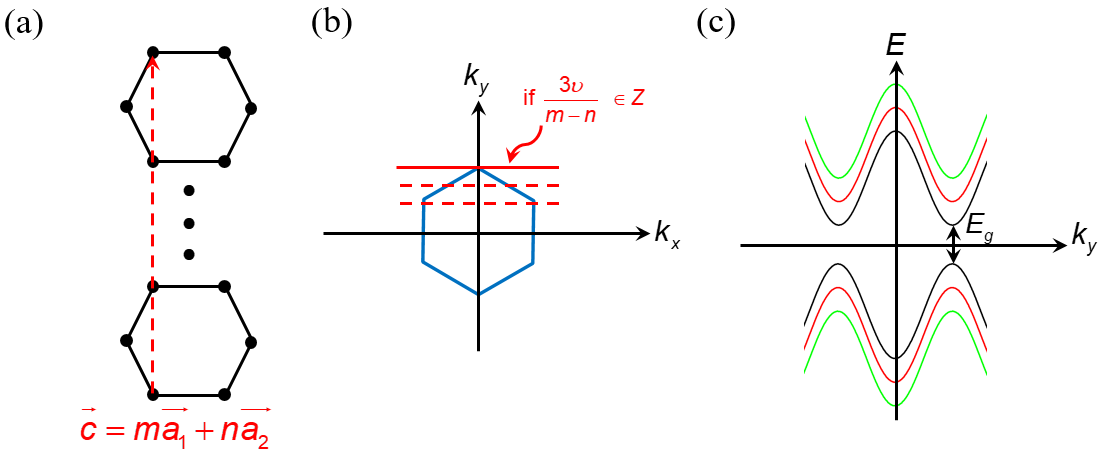
\includegraphics[width=0.9\textwidth]{figures/Fig2_8}
\centering
\caption{\small (a) Illustration of rolling a zigzag nanotube. (b) Brillouin zone and possible solutions (straight lines) of zigzag nanotube. (c) $E-k_{y}$ diagram when $(m-n)$ is not an integer multiple of 3.}
\end{figure} Because now the wavefunction is restricted in $y$-direction, the $k_{x}$ is zero and thus the Equation (2.89) becomes \begin{equation}
    k_{y} = \frac{2\pi}{3b}\frac{3\nu}{m-n}
\end{equation} If $\frac{3\nu}{m-n}$ is an integer, the zigzag nanotube will become metallic since $k_{y}$ crosses the corner of Brillouin zone [see Fig. 2.8(b)]. If $\frac{3\nu}{m-n}$ is not an integer, the zigzag nanotube behaves like a semiconductor and there is a bandgap $E_{g}$ as shown in Fig. 2.8(c). The bandgap can be evaluated using the Equation (2.85) \begin{align}
    E_{g}& = 2\times\frac{3}{2}a_{0}t\sqrt{k_{x}^{2}+\left(k_{y}\mp\frac{2\pi}{3b}\right)^{2}}\big|_{k_{x}=0,k_{y}=\frac{2\pi}{3b}\frac{3\nu}{m-n}}\nonumber\\
    & = 3a_{0}t\frac{3}{m-n}\left(\nu\mp\frac{m-n}{3}\right)\frac{2\pi}{3b}\nonumber\\
    &\xrightarrow{minimum} 3a_{0}t\frac{3}{m-n}\frac{1}{3}\frac{2\pi}{3b} = \frac{2a_{0}t\pi}{\left(m-n\right)b}
\end{align} If the diameter of the zigzag nanotube is $d$, the bandgap is \begin{equation}
    E_{g} = \frac{2a_{0}t}{d} = \frac{0.8}{d\text{ (nm)}}\text{ eV}
\end{equation} where $\pi d = (m-n)b$. The Equation (2.93) is validated by the experimental results. However, if $d<1$ nm, it is not accurate (but the trend is still correct) due to the presence of strain.

\chapter{Scattering}
\section{Free Electron}
Suppose there is an electron traveling with a momentum $k$ without experiencing the potential energy ($U=0$). At $t=0$, the scattering happens and the momentum changes from $k$ to $k'$ as shown in Fig. 3.1.
\begin{figure}[tbp]
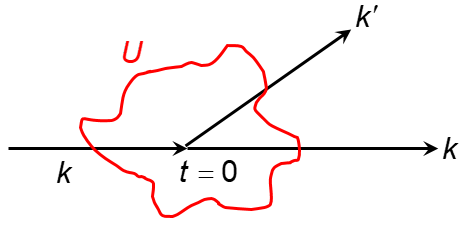
\includegraphics[width=0.4\textwidth]{figures/Fig3_1}
\centering
\caption{\small The electron with a momentum $k$ and the scattering happens at $t = 0$.}
\end{figure}
Thus, \begin{align}
    \big|\psi(x,t)\big>& = \sum_{k}{c_{k}(t)}\big|\phi_{k}(x)\big>\nonumber\\
    & = c_{k}(t)\big|\phi_{k}(x)\big>\text{,}\quad\text{$t=0$}\nonumber\\
    & = \big|\phi_{k}(x)\big> = e^{ikx}
\end{align} where \begin{equation}
    c_{k}(0)=
    \begin{cases}
    1 & \text{for momentum$=k$ since we already knew $k$}\\
    0 & \text{for every other momentum}
    \end{cases}
\end{equation} The Schrodinger equation tells \begin{equation}
    i\hbar\frac{\partial}{\partial t}\big|\psi(x,t)\big> = -\frac{\hbar^{2}}{2m_{0}}\nabla^{2}\big|\psi(x,t)\big>\nonumber
\end{equation} \begin{equation}
    \Rightarrow\sum_{k}{i\hbar\frac{\partial}{\partial t}c_{k}\big|\phi_{k}(x,t)\big>} = \sum_{k}{-\frac{\hbar^{2}}{2m_{0}}\nabla^{2}c_{k}\big|\phi_{k}(x,t)\big>}\nonumber
\end{equation} \begin{equation}
    \Rightarrow\sum_{k}{\big|\phi_{k}(x,t)\big>i\hbar\frac{\partial}{\partial t}c_{k}} = \sum_{k}{c_{k}\varepsilon_{k}\big|\phi_{k}(x,t)\big>}
\end{equation} $\big<\phi_{k}'(x,t)\big|$: \begin{equation}
    i\hbar\frac{\partial}{\partial t}c_{k'} = c_{k'}\varepsilon_{k'}\nonumber
\end{equation} \begin{equation}
    \Rightarrow\frac{\partial}{\partial t}c_{k'} = -i\omega_{k'}c_{k'}\nonumber
\end{equation} \begin{equation}
    \Rightarrow\boxed{c_{k'}(t) = c_{k'}(0)e^{-i\omega_{k'}t}}
\end{equation}
\section{Electron Experiencing Potential}
If $U\neq 0$ and is a function of both position $x$ and time $t$, the Schrodinger's equation becomes \begin{equation}
    i\hbar\frac{\partial}{\partial t}c_{k}(t)\big|\phi_{k}(x)\big> = -\frac{\hbar^{2}}{2m_{0}}\nabla^{2}c_{k}(t)\big|\phi_{k}(x)\big> + Uc_{k}(t)\big|\phi_{k}(x)\big>
\end{equation} $\big<\phi_{k}'(x,t)\big|$: \begin{equation}
    i\hbar\frac{\partial}{\partial t}c_{k'} = c_{k'}\varepsilon_{k'} + \sum_{k}{\big<\phi_{k'}\big|U\big|\phi_{k}\big>c_{k}}
\end{equation} If $\big<\phi_{k'}\big|U\big|\phi_{k}\big>\equiv U_{k'k}(t)$ and $\frac{\varepsilon_{k'}}{\hbar}\equiv \omega_{k'}$, then \begin{equation}
    \boxed{\frac{\partial}{\partial t}c_{k'} + i\omega_{k'}c_{k'} = \frac{1}{i\hbar}\sum_{k}{U_{k'k}c_{k}}}
\end{equation} The general solution of the Equation (3.7) is \begin{equation}
    c_{k'}(T) = e^{-i\omega_{k'}T}\int_{0}^{T}dt\sum_{k}{\frac{U_{k'k}}{i\hbar}c_{k}e^{i\omega_{k'}t}}
\end{equation} Since the solution $c_{k'}$ contains itself $c_{k}$, the iteration is needed to get $c_{k'}$. Here, we adopt the $c_{k}$ for the free electron Hamiltonian [Equation (3.4)] as a first-order approximation. Thus, \begin{equation}
    \boxed{c_{k'}(T) = e^{-i\omega_{k'}T}\int_{0}^{T}dt\sum_{k}{\frac{U_{k'k}}{i\hbar}e^{i(\omega_{k'}-\omega_{k})t}}}
\end{equation} The scattering probability $P_{k'k}^{T}$ is \begin{equation}
    P_{k'k}^{T} = c_{k'}c_{k} = \frac{1}{\hbar^{2}}\big|\int_{0}^{T}\sum_{k}{U_{k'k}e^{i(\omega_{k'}-\omega_{k})t}}dt\big|^{2}
\end{equation} and the scattering rate $S_{k'k}$ is\footnote{The same results can be obtained using the {\bf Perturbation Theory}. In fact, the first order approximation used in the Equation (3.9) is the perturbation theory itself.} \begin{equation}
    \boxed{S_{k'k} = \frac{P_{k'k}^{T}}{T} = \frac{1}{T\hbar^{2}}\big|\int_{0}^{T}\sum_{k}{U_{k'k}e^{i(\omega_{k'}-\omega_{k})t}}dt\big|^{2}}
\end{equation}
\subsubsection{If $U_{k'k}$ is only a function of $x$}
In practical cases, this approximation is valid since the impurities cannot move in the solids. The $U_{k'k}$ can be taken out from the integration in the Equation (3.11). Thus, \begin{equation}
    S_{k'k} = \frac{1}{T\hbar^{2}}\sum_{k}\big|U_{k'k}\big|^{2}\big|\int_{0}^{T}e^{i\omega t}dt\big|^{2}
\end{equation} where $\omega \equiv \omega_{k'}-\omega_{k}$. The integration in the Equation (3.12) can be evaluated analytically\footnote{This is not a delta function since $T$ is not infinity.} \begin{align}
    \big|\int_{0}^{T}e^{i\omega t}dt\big|^{2}& = \big|\int_{0}^{T}(\cos{\omega t}+i\sin{\omega t})dt\big|^{2}\nonumber\\
    & = \frac{2}{\omega^{2}}(1-\cos{\omega T}) = \frac{\sin{\frac{\varepsilon T}{2\hbar}}^{2}}{(\frac{\varepsilon T}{2\hbar})^{2}}T^{2}
\end{align} where $\varepsilon \equiv \hbar \omega$. The function of $\frac{\sin{x}^{2}}{x^{2}}$ is shown in Fig. 3.2.
\begin{figure}[tbp]
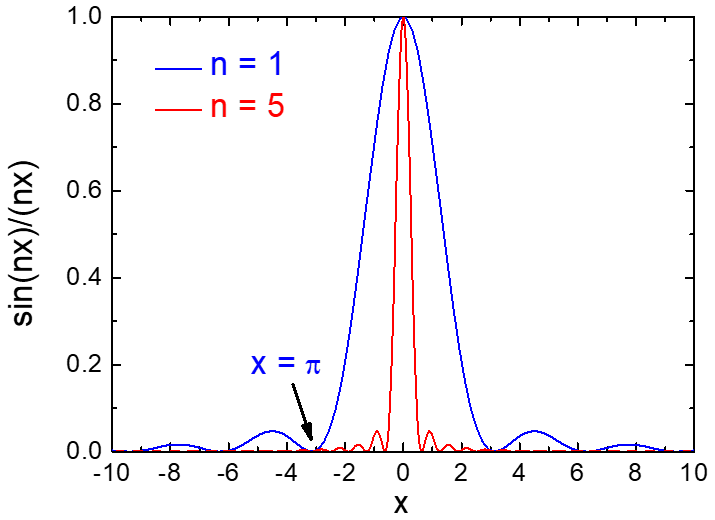
\includegraphics[width=0.6\textwidth]{figures/Fig3_2}
\centering
\caption{\small $\frac{\sin{nx}}{nx}$ versus $x$ at $n = 1$ and $5$. When $n$ is large, the function approaches to the delta function. In other words, if $\frac{\varepsilon T}{2\hbar}\gg\pi$, $\frac{\sin{x}}{x}$ becomes the delta function.}
\end{figure}
When $T \gg \frac{2\pi\hbar}{\varepsilon} ~ \text{f-sec}$, $\frac{\sin{\frac{\varepsilon T}{2\hbar}}^{2}}{(\frac{\varepsilon T}{2\hbar})^{2}}$ can be approximated as a delta function. This approximation is valid in electronics since the scattering time is in order of p-sec. However, in optoelectronics, this approximation is not good because the scattering time as faster as f-sec is possible. To ensure that the integration is not changed after replacing $\frac{\sin{\frac{\varepsilon T}{2\hbar}}^{2}}{(\frac{\varepsilon T}{2\hbar})^{2}}$ with a delta function, the area under the function should be obtained \begin{equation}
    \int \frac{\sin{\frac{\varepsilon T}{2\hbar}}^{2}}{(\frac{\varepsilon T}{2\hbar})^{2}}d\varepsilon = \int \frac{\sin{x}^{2}}{x^{2}}dx \frac{2\hbar}{T}
\end{equation} The above equation can be evaluated using the following trick \begin{equation}
    I(a)\equiv \int\frac{\sin{ax}^{2}}{x^{2}}dx
\end{equation} \begin{equation}
    \frac{dI}{da} = 2\int \frac{\sin{ax}}{x}dx = \pi \Rightarrow I(a) = a\pi
\end{equation} Then, \begin{equation}
    \int \frac{\sin{x}^{2}}{x^{2}}dx \frac{2\hbar}{T} = \frac{2\pi\hbar}{T}
\end{equation} Thus, \begin{equation}
    S_{k'k} = \frac{1}{T\hbar^{2}}\frac{2\pi\hbar}{T}\sum_{k}{\big|U_{k'k}\big|^{2}\delta(\varepsilon_{k'}-\varepsilon_{k})}T^{2}\nonumber
\end{equation}
Or \begin{equation}
    \boxed{S_{k'k} = \frac{2\pi}{\hbar}\sum_{k}{\big|U_{k'k}\big|^{2}\delta(\varepsilon_{k'}-\varepsilon_{k})}}
\end{equation} which is called the {\bf Fermi Golden Rule}. From the above equation, if the potential is time-independent, the scattering will be elastic without losing or gaining any energy.
\subsubsection{If $U_{k'k}$ is only a function of $t$}
If the solid is illuminated by the light or is emitting the photons, the potential will be time-dependent. The potential $U_{k'k}$ can be generally expanded by the Fourier series \begin{equation}
    U_{k'k} = g(t) = \sum_{\omega}{g_{\omega}e^{i\omega t}} + \sum_{\omega}{g_{-\omega}e^{-i\omega t}}
\end{equation} Then, \begin{align}
    S_{k'k}& = \frac{1}{T\hbar^{2}}\sum_{k,\omega}{\big|g_{\omega}^{k'k}\big|^{2}\big|\int_{0}^{T}e^{i(\omega_{k'}-\omega_{k}+\omega)t}dt\big|^{2}+\big|g_{-\omega}^{k'k}\big|^{2}\big|\int_{0}^{T}e^{i(\omega_{k'}-\omega_{k}-\omega)t}dt\big|^{2}}\nonumber\\
    & = \frac{2\pi}{\hbar}\sum_{k,\omega}{\big|g_{\omega}^{k'k}\big|^{2}\delta(\varepsilon_{k'}-\varepsilon_{k}+\hbar\omega)}+\frac{2\pi}{\hbar}\sum_{k,\omega}{\big|g_{-\omega}^{k'k}\big|^{2}\delta(\varepsilon_{k'}-\varepsilon_{k}-\hbar\omega)}
\end{align} The first term in the Equation (3.20) represents the emission process since \begin{equation}
    \varepsilon_{k'} = \varepsilon_{k} - \hbar\omega \nonumber
\end{equation} and the second term represents the absorption process since \begin{equation}
    \varepsilon_{k'} = \varepsilon_{k} + \hbar\omega \nonumber
\end{equation} Note that the cross term in the Equation (3.20) is ignored since physically the absorption and emission processes cannot happen simultaneously.
\section{Master Equation}
Since the scattering changes the momentum from $k$ to $k'$, the distribution function of the electron also changes obeying the {\bf Mater Equation} \begin{equation}
    \frac{df_{k}}{dt} = \sum_{k'}{S_{kk'}f_{k'}(1-f_{k})} - \sum_{k'}{S_{k'k}f_{k}(1-f_{k'})}
\end{equation} where the first and second terms on the right side represent the scattering from $k'$ to $k$ and from $k$ to $k'$. At equilibrium, $\frac{df_{k}}{dt}=0$. Thus, \begin{equation}
    S_{kk'}f_{k'}(1-f_{k}) = S_{k'k}f_{k}(1-f_{k'})\nonumber
\end{equation} or, \begin{align}
    \frac{S_{kk'}}{S_{k'k}}& = \frac{\frac{f_{k}}{1-f_{k}}}{\frac{f_{k'}}{1-f_{k'}}} = \frac{e^{-(\varepsilon_{k}-\mu)/k_{B}T}}{e^{-(\varepsilon_{k'}-\mu)/k_{B}T}} = e^{(\varepsilon_{k'}-\varepsilon_{k})/k_{B}T} = e^{\hbar\omega/k_{B}T}
\end{align} where $f_{k} = 1/[1+e^{(\varepsilon_{k}-\mu)/k_{B}T}]$ and $\varepsilon_{k'}-\varepsilon_{k}\equiv \hbar\omega$. The Equation (3.22) indicates the restoration of the equilibrium. In other words, the probability of going from the higher energy state to the lower is proportional to $e^{\hbar\omega/k_{B}T}$. Recall the Equation (3.20). The emission and absorption have a similar relation \begin{equation}
    \frac{\big|g_{\omega}\big|^{2}}{\big|g_{-\omega}\big|^{2}} = e^{\hbar\omega/k_{B}T}
\end{equation} Since $f_{k}$ is not a function of $k'$, it can be taken out from the summation. Thus, the Master equation becomes \begin{equation}
    \boxed{\frac{df_{k}}{dt} + \frac{f_{k}}{\tau} = \sum_{k'}{S_{kk'}f_{k'}(1-f_{k})}}
\end{equation} where \begin{equation}
    \frac{1}{\tau} = \sum_{k'}{S_{k'k}(1-f_{k'})}
\end{equation} is the lifetime ($\tau$) of the electron due to the scattering. The general solution of the Equation (3.24) is \begin{equation}
    f_{k} = e^{-T/\tau}\int_{0}^{T}e^{t/\tau}\sum_{k'}{S_{kk'}f_{k'}(1-f_{k})}dt
\end{equation} Again, the Equation (3.26) needs to be solved numerically. Let's consider a simplified case: if an electron is coming with the momentum $k$, we have \begin{equation}
    \begin{cases}
    f_{k} = 1 & \text{for momentum$=k$ since we already knew $k$}\\
    f_{k'} = 0 & \text{for every other momentum $k'$}
    \end{cases}
\end{equation} Thus, \begin{equation}
    1-f_{k}\approx 0 \Rightarrow \frac{df_{k}}{dt} + \frac{f_{k}}{\tau} = 0 \Rightarrow f_{k}(t) = f_{k}(0)e^{-t/\tau}
\end{equation}
\section{Relaxation Time}
The relaxation time is the time that a physical quantity $\vec{A}$ is back to the thermal equilibrium and follows \begin{equation}
    \frac{d\big<\vec{A}\big>}{dt} = \frac{\big<\vec{A}\big>-\big<\vec{A_{0}}\big>}{\tau_{A}}
\end{equation} where $\tau_{A}$ is the relaxation time and \begin{equation}
    \big<\vec{A}\big> = \big<\psi\big|A\big|\psi\big> = \text{Trace}(A\rho)
\end{equation} Assume that there is no off-diagonal elements \begin{equation}
    \big<A\big>_{k} = \big<\psi_{k}\big|A\big|\psi_{k}\big> = f_{k}A_{k}
\end{equation} Thus, \begin{equation}
    \frac{d\big<\vec{A}\big>}{dt} = \frac{d}{dt}\sum_{k}{\big<A\big>_{k}} = \frac{d}{dt}\sum_{k}{f_{k}A_{k}}
\end{equation} Multiplying $\sum_{k}{A_{k}}$ to the Master equation, we have \begin{align}
    \sum_{k}{\frac{d}{dt}f_{k}A_{k}}& = \sum_{kk'}{\underbrace{S_{kk'}f_{k'}(1-f_{k})A_{k}}_{=S_{k'k}f_{k}(1-f_{k'})A_{k'}}} - \sum_{kk'}{S_{k'k}f_{k}(1-f_{k'})A_{k}}\nonumber\\
    & = \sum_{kk'}{S_{k'k}f_{k}(1-f_{k'})[A_{k'}-A_{k}]} = \frac{\big<\vec{A}\big>-\big<\vec{A_{0}}\big>}{\tau_{A}}
\end{align} Hence, \begin{align}
    \frac{1}{\tau_{A}}& = \frac{\sum_{kk'}{S_{k'k}f_{k}(1-f_{k'})[A_{k'}-A_{k}]}}{\big<\vec{A}\big>-\big<\vec{A_{0}}\big>}\nonumber\\
    & = \frac{\sum_{kk'}{S_{k'k}f_{k}(1-f_{k'})[A_{k'}-A_{k}]}}{\sum_{k}{f_{k}A_{k}}-\sum_{k}{f_{k0}A_{k}}}\nonumber\\
    & = \frac{\sum_{kk'}{S_{k'k}f_{k}(1-f_{k'})}}{\sum_{k}{f_{k}-f_{k0}}}\left[1-\frac{A_{k'}}{A_{k}}\right]\nonumber\\
    & = \sum_{k}{\frac{1}{\tau_{A}}(k)}
\end{align} where $\frac{1}{\tau_{k}}(k)$ is the $k$-dependent relaxation time \begin{equation}
    \boxed{\frac{1}{\tau_{A}}(k) = \sum_{k'}{\frac{S_{k'k}f_{k}(1-f_{k'})}{f_{k}-f_{k0}}\left[1-\frac{A_{k'}}{A_{k}}\right]}}
\end{equation}
\section{Phonons}
The phonons are the quantized quasi-particles that represent the lattice vibration. The one-dimensional lattice can be modeled as the atoms connected to each other by the springs as shown in Fig. 3.3.
\begin{figure}[tbp]
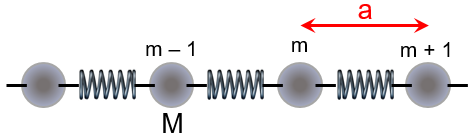
\includegraphics[width=0.6\textwidth]{figures/Fig3_3}
\centering
\caption{\small One dimensional lattice (lattice constant is $a$) with the springs connecting each atom with the mass $M$.}
\end{figure}
The force equation says \begin{equation}
    F = M\frac{d^{2}x_{m}}{dt^{2}} = K\left[(x_{m+1}-x_{m})-(x_{m}-x_{m-1})\right]
\end{equation} where $K$ is the spring constant and the $x$ is the position of the atom. The solution of the Equation (3.36) is \begin{align}
    \widetilde{x_{m}}& = \widetilde{x}e^{i(\beta ma - \omega t)} + \widetilde{x}^{*}e^{-i(\beta ma - \omega t)}\nonumber\\
    & = 2\big|\widetilde{x}\big|\cos{(\beta ma - \omega t + \phi)} \equiv 2\big|\widetilde{x}\big|\cos{\theta}
\end{align} where $\widetilde{x}$ is the amplitude, $\beta$ is the momentum, and $phi$ is the phase. To determine the dispersion relation of phonons, we take the derivative to the Equation (3.37) with respect to time $t$ twice and equate it to the Equation (3.36) \begin{equation}
    2\big|\widetilde{x_{m}}\big|(-\cos{\theta})(-\omega)(-\omega) = -\frac{K}{M}2\big|\widetilde{x_{m}}\big|4\cos{\theta}\sin^{2}{\frac{\beta a}{2}}
\end{equation} Thus, the dispersion relation is \begin{equation}
    \boxed{\omega(\beta) = 2\sqrt{\frac{K}{M}}\sin{\frac{\beta a}{2}}}
\end{equation} When $\omega$ is close to zero, the Equation (3.39) can be expanded as a straight line. In other words, \begin{equation}
    \omega \propto \beta \quad \Rightarrow \quad \omega = c_{S}\beta
\end{equation} where $c_{S}$ is the velocity of sound since the Equation (3.39) represents the acoustic phonon mode where all the atoms move in the same direction. For optical phonon mode, the frequency $\omega$ is nearly a constant say $\omega_{0}$ and the two atoms move in the opposite direction. The kinetic energy of an atom in the acoustic mode at momentun $\beta$ is \begin{equation}
    \frac{1}{2}Mv^{2} = 2M\big|\widetilde{x_{\beta}}\big|^{2}\omega_{\beta}^{2}\sin^{2}{(\overset{\rightharpoonup}{\beta}\cdot\overset{\rightharpoonup}{r}-\omega_{\beta}t)}
\end{equation} If there are $N$ atoms, the total energy will be \begin{align}
    E^{\text{total}}& = 2M\big|\widetilde{x_{\beta}}\big|^{2}\omega_{\beta}^{2}N,\quad MN\equiv \rho V \nonumber\\
    & = 2\rho V \big|\widetilde{x_{\beta}}\big|^{2}\omega_{\beta}^{2}\nonumber\\
    & = n_{\beta}\hbar\omega_{\beta}
\end{align} where $\rho$ is the mass density and $n_{\beta}$ is the number of phonons (fermion) \begin{equation}
    n_{\beta} = \frac{1}{e^{\frac{\hbar\omega_{\beta}}{k_{B}T}}-1}
\end{equation} Hence, \begin{equation}
    \big|\widetilde{x_{\beta}}\big|^{2} = \frac{\hbar n_{\beta}}{2\rho V \omega_{\beta}}
\end{equation} and \begin{equation}
    \widetilde{x_{\beta}}(\overset{\rightharpoonup}{r},t) = \sqrt{\frac{\hbar}{2\rho V\omega_{\beta}}}\left[a_{\beta}e^{i(\overset{\rightharpoonup}{\beta}\cdot\overset{\rightharpoonup}{r}-\omega_{\beta}t)}+a_{\beta}^{*}e^{-i(\overset{\rightharpoonup}{\beta}\cdot\overset{\rightharpoonup}{r}-\omega_{\beta}t)}\right]
\end{equation} where \begin{equation}
    a_{\beta}^{*}a_{\beta} = n_{\beta} = \frac{1}{e^{\frac{\hbar\omega_{\beta}}{k_{B}T}}-1}
\end{equation}
\subsection{Electron-Phonon Scattering}
The electron-phonon scattering potential $U_{\beta}^{S}$ can be approximated as \begin{align}
    U_{\beta}^{S}(\overset{\rightharpoonup}{r},t) = K_{\beta}\widetilde{x_{\beta}}(\overset{\rightharpoonup}{r},t)
\end{align} where $K_{\beta}$ is the coupling constant related to the deformation of the lattice. For the acoustic mode, the movement of the atoms imposes the strain on the lattice, and thus \begin{equation}
    U_{\beta}^{S} = D_{a}S_{\beta} = D_{a}(\nabla\cdot\widetilde{x_{\beta}}) = i\beta D_{a}\widetilde{x_{\beta}} \equiv K_{\beta}\widetilde{x_{\beta}}
\end{equation} where $D_{a}$ is the deformation potential and $S_{\beta}$ is the strain. The Equation (3.47) is the result of the Taylor expansion of change in the potential. For the optical phonon mode, the frequency is nearly fixed. Thus, \begin{equation}
    K_{\beta} = D_{o}
\end{equation} Since we assume the phonon modes ($\phi_{k}$) are the plane waves\footnote{S. Datta, Quantum Transport Atom to Transistor, 2005, p. 261.}, we have \begin{align}
    U_{k'k}(t)& = \big<\phi_{k'}\big|U_{\beta}^{S}(\overset{\rightharpoonup}{r},t)\big|\phi_{k}\big>\nonumber\\
    & = K_{\beta}\sqrt{\frac{\hbar}{2\rho V\omega_{\beta}}}\left(\underbrace{\int a_{\beta}^{*}e^{-\overset{\rightharpoonup}{k'}\cdot\overset{\rightharpoonup}{r}}e^{\overset{\rightharpoonup}{-\beta}\cdot\overset{\rightharpoonup}{r}}e^{\overset{\rightharpoonup}{k}\cdot\overset{\rightharpoonup}{r}}e^{i\omega_{\beta}t}}_{\text{emission}}+\underbrace{\int a_{\beta}e^{-\overset{\rightharpoonup}{k'}\cdot\overset{\rightharpoonup}{r}}e^{\overset{\rightharpoonup}{\beta}\cdot\overset{\rightharpoonup}{r}}e^{\overset{\rightharpoonup}{k}\cdot\overset{\rightharpoonup}{r}}e^{-i\omega_{\beta}t}}_{\text{absorption}}\right)
\end{align} and \begin{equation}
    \big|U_{k'k}\big|^{2} = \underbrace{\big|K_{\beta}\big|^{2}\frac{\hbar a_{\beta}a_{\beta}^{*}}{2\rho V\omega_{\beta}}\delta(\overset{\rightharpoonup}{k}-\overset{\rightharpoonup}{k'}-\overset{\rightharpoonup}{\beta})}_{\text{emission}}+\underbrace{\big|K_{\beta}\big|^{2}\frac{\hbar a_{\beta}^{*}a_{\beta}}{2\rho V\omega_{\beta}}\delta(\overset{\rightharpoonup}{k}-\overset{\rightharpoonup}{k'}+\overset{\rightharpoonup}{\beta})}_{\text{absorption}}
\end{equation} From the Equation (3.23), we have\footnote{Conceptually, $a_{\beta}a_{\beta}^{*}$ and $a_{\beta}^{*}a_{\beta}$ are the {\bf lowering operator} and {\bf raising operator} of the simple harmonic oscillator which satisfies $[a_{\beta}a_{\beta}^{*},a_{\beta}^{*}a_{\beta}] = 1$ and thus $a_{\beta}^{*}a_{\beta}=n_{\beta}+1$. See D. J. Griffiths, Introduction to Quantum Mechanics, 2005, p. 43-44.} \begin{equation}
    \frac{\text{emission}=a_{\beta}a_{\beta}^{*}}{\text{absorption}=a_{\beta}^{*}a_{\beta}=n_{\beta}} = e^{\hbar\omega/kT}\quad\Rightarrow\quad a_{\beta}^{*}a_{\beta}=n_{\beta}+1
\end{equation} Therefore, the scattering rate [the Equation (3.20)] becomes \begin{align}
    S_{k'k}& = \underbrace{\sum_{k,\beta}{\frac{\pi(n_{\beta}+1)}{\rho V \omega_{\beta}}\big|K_{\beta}\big|^{2}\delta(\overset{\rightharpoonup}{k}-\overset{\rightharpoonup}{k'}-\overset{\rightharpoonup}{\beta})\delta(\varepsilon_{k'}-\varepsilon_{k}+\hbar\omega_{\beta})}}_{\text{emission}}\nonumber\\
    &\quad +\underbrace{\sum_{k,\beta}{\frac{\pi n_{\beta}}{\rho V \omega_{\beta}}\big|K_{\beta}\big|^{2}\delta(\overset{\rightharpoonup}{k}-\overset{\rightharpoonup}{k'}+\overset{\rightharpoonup}{\beta})\delta(\varepsilon_{k'}-\varepsilon_{k}-\hbar\omega_{\beta})}}_{\text{absorption}}
\end{align} Note that at $T=0$K, the absorption $n_{\beta} = 0$ but the emission $n_{\beta}+1\neq 0$, indicating the spontaneous emission.
\subsection{Simplification of Electron-Phonon Scattering Using Effective Mass Approximation}
Since the Equation (3.53) involves the electronic band structure effect, it's difficult to solve in the real device geometry. Thus, the effective mass approximation is applied to simplify the problem. In the Equation (3.53), the momentum is conserved with the phonon momentum, so the momentum of the emission and absorption processes can be drawn as shown in Fig. 3.4.
\begin{figure}[tbp]
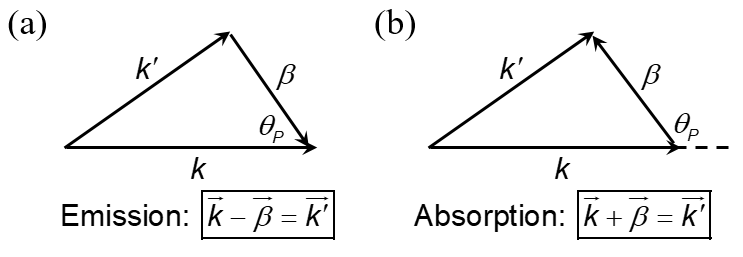
\includegraphics[width=0.6\textwidth]{figures/Fig3_4}
\centering
\caption{\small (a) Phonon emission and (b) absorption processes.}
\end{figure}
From the energy conservation of the emission process, we have \begin{equation}
    \varepsilon_{k'}-\varepsilon_{k}+\hbar\omega_{\beta} = 0\nonumber
\end{equation} \begin{equation}
    \Rightarrow \frac{\hbar^{2}}{2m}\left(k'^{2}-k^{2}+\frac{2m\omega_{\beta}}{\hbar}\right) = 0, \quad k'^{2} = k^{2}+\beta^{2}-2k\beta\cos{\theta_{P}}\nonumber
\end{equation} \begin{equation}
    \Rightarrow \boxed{\cos{\theta_{P}} = \frac{m\omega_{\beta}}{\hbar k \beta}+\frac{\beta}{2k}} \quad \text{For emission}
\end{equation} Similarly, \begin{equation}
    \boxed{\cos{\theta_{P}} = \frac{m\omega_{\beta}}{\hbar k \beta}-\frac{\beta}{2k}} \quad \text{For absorption}
\end{equation}
\subsubsection{Acoustic Phonon}
For acoustic phonon, the dispersion relation can be simplified as [Equation (3.40)]\begin{equation}
    \omega_{\beta} = c_{S}\beta\nonumber
\end{equation} Thus, the momentum $\beta$ for the emission and absorption are \begin{equation}
    \beta^{\text{em}} = 2k\left(\cos{\theta_{P}}-\frac{mc_{S}}{\hbar k}\right)
\end{equation} \begin{equation}
    \beta^{\text{ab}} = 2k\left(\frac{mc_{S}}{\hbar k}-\cos{\theta_{P}}\right)
\end{equation} Since $\cos{\theta_{P}}\leq 1$, for the emission to happen we have \begin{equation}
    \frac{mc_{S}}{\hbar k}<1\quad\Rightarrow\quad\frac{\hbar k}{m}>c_{S}
\end{equation} which is the Cherenkov condition saying that the velocity of the electron should be greater than the sound velocity to emit the acoustic phonon.
\subsubsection{Optical Phonon}
Since the frequency in the optical phonon mode is nearly fixed, we have \begin{equation}
    \cos{\theta_{P}} = \frac{m\omega_{0}}{\hbar k \beta^{\text{em}}}+\frac{\beta^{\text{em}}}{2k}
\end{equation} for the emission. Hence, \begin{equation}
    \beta^{\text{em}} = k\cos{\theta_{P}}\pm\sqrt{k^{2}\cos^{2}{\theta_{P}}-\frac{2m\omega_{0}}{\hbar}}
\end{equation} Since $\cos{\theta_{P}}\leq 1$, for the emission to happen we have \begin{equation}
    \frac{2m\omega_{0}}{\hbar} < k^{2}\quad\Rightarrow\quad\frac{\hbar^{2}k^{2}}{2m}>\hbar\omega_{0}
\end{equation} indicating that the kinetic energy of the electron should be larger than that of the optical phonon for the emission.
\subsubsection{Lifetime of Electron-Phonon Scattering}
If the condition $\overset{\rightharpoonup}{k}-\overset{\rightharpoonup}{k'}\pm\overset{\rightharpoonup}{\beta}=0$ has been held, the Equation (3.53) can be further simplified using the effective mass approximation \begin{align}
    S_{k'k}(k)& = \underbrace{\frac{\pi m}{\rho V\hbar^{2}}\sum_{\beta}{\frac{\big|K_{\beta}\big|^{2}(n_{\beta}+1)}{ \omega_{\beta}k\beta}\delta\left(\cos{\theta_{P}}-\frac{m\omega_{\beta}}{\hbar k\beta}-\frac{\beta}{2k}\right)}}_{\text{emission}}\nonumber\\
    &\quad +\underbrace{\frac{\pi m}{\rho V\hbar^{2}}\sum_{\beta}{\frac{\big|K_{\beta}\big|^{2}n_{\beta}}{ \omega_{\beta}k\beta}\delta\left(\cos{\theta_{P}}-\frac{m\omega_{\beta}}{\hbar k\beta}+\frac{\beta}{2k}\right)}}_{\text{absorption}}
\end{align} Recall the Equations (3.25), (3.27), and (3.28), the lifetime of the electron-phonon scattering is\footnote{Summing over $k'$ is the same as summing over $\beta$.} \begin{equation}
    \frac{1}{\tau(k)} = \sum_{\beta}{S_{k'k}^{\text{em}}}+\sum_{\beta}{S_{k'k}^{\text{ab}}}
\end{equation} and the summation over $\beta$ is \begin{equation}
    \sum_{\beta} \rightarrow \int\frac{d\beta_{x}d\beta_{y}d\beta_{z}}{\frac{2\pi}{L_{x}}\frac{2\pi}{L_{y}}\frac{2\pi}{L_{z}}} = \frac{V}{8\pi^{3}}\int\beta^{2}d\beta(2\pi)\int_{-1}^{1}d\cos{\theta_{P}}
\end{equation} The lifetime of the acoustic phonon emission is \begin{align}
    \frac{1}{\tau^{\text{em}}(k)}& = \frac{\pi m}{\rho V\hbar^{2}}\frac{V}{8\pi^{3}}2\pi\int_{\beta_{\text{min}}}^{\beta_{\text{max}}}\frac{\beta^{2}d\beta\big|K_{\beta}\big|^{2}(n_{\beta}+1)}{\omega_{\beta}k\beta}\int_{-1}^{1}\delta\left(\cos{\theta_{P}}-\frac{m\omega_{\beta}}{\hbar k\beta}-\frac{\beta}{2k}\right)d\cos{\theta_{P}}\nonumber\\
    & = \frac{mD_{a}^{2}}{4\pi\rho\hbar^{2}}\frac{1}{kc_{S}}\int_{\beta_{\text{min}}}^{\beta_{\text{max}}}\beta^{2}d\beta(n_{\beta}+1),\quad \omega_{\beta}=c_{S}\beta\quad\text{and}\quad\big|K_{\beta}\big|^{2}=\beta^{2}D_{a}^{2}
\end{align} For the acoustic phonon, $\hbar\omega_{\beta}\ll k_{B}T$, and thus $n_{\beta}\approx\frac{k_{B}T}{\hbar\omega_{\beta}}\gg 1$ and $n_{\beta}+1\approx n_{\beta}$. Furthermore, $\beta_{\text{max}}^{\text{em}}\approx 2k$ and $\beta_{\text{min}}^{\text{em}}\approx 0$. The Equation (3.65) becomes \begin{align}
    \frac{1}{\tau^{\text{em}}(k)}& = \frac{mD_{a}^{2}}{4\pi\rho\hbar^{3}}\frac{k_{B}T}{kc_{S}^{2}}\int_{0}^{2k}\beta d\beta = \frac{mD_{a}^{2}k_{B}T}{2\pi\rho\hbar^{3}c_{S}^{2}}k
\end{align} Similarly, the lifetime of the absorption is \begin{equation}
    \frac{1}{\tau^{\text{ab}}(k)} = \frac{mD_{a}^{2}k_{B}T}{2\pi\rho\hbar^{3}c_{S}^{2}}k
\end{equation} Therefore, the total lifetime due to the electron-phonon scattering is \begin{align}
    \frac{1}{\tau(k)}& = \frac{mD_{a}^{2}k_{B}T}{\pi\rho\hbar^{3}c_{S}^{2}}k,\quad k=\frac{\sqrt{2mE(k)}}{\hbar}\nonumber\\
    & = \frac{(2mk_{B}T)^{3/2}D_{a}^{2}}{2\pi\rho\hbar^{4}c_{S}^{2}}\sqrt{\frac{E(k)}{k_{B}T}}
\end{align} For GaAs, \begin{equation}
    \tau = 7.6\sqrt{\frac{k_{B}T}{E}}\quad\text{psec}\nonumber
\end{equation}
\chapter{Semiclassical Transport}
\section{Boltzmann Transport Equation}
In Chapter 2, we've discussed how to calculate the current with the Hamiltonian of the material. However, the brute force of solving this complicated problem is numerically inefficient. Therefore, a semiclassical way, which includes the quantum mechanical correction, is desired. The Fermi distribution can be written as \begin{equation}
    f_{k} = \frac{1}{1+e^{(E_{k}-\mu)/(k_{B}T)}} = \frac{1}{1+e^{(\frac{P^{2}}{2m}-\mu)/(k_{B}T)}}
\end{equation} Since $p = \hbar k$, the $f_{k}$ in general is shown in Fig. 4.1.
\begin{figure}[tbp]
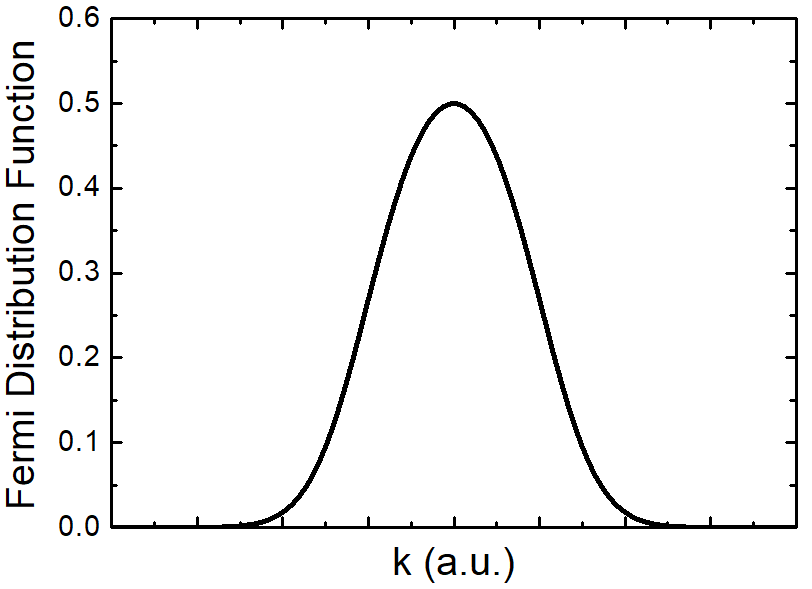
\includegraphics[width=0.4\textwidth]{figures/Fig4_1}
\centering
\caption{\small Fermi distribution function as a function of $k$.}
\end{figure}
The $f_{k}$ can be further extended into space-, momentum-, and time-dependence, i.e., \begin{equation}
    f_{k} = g(\overset{\rightharpoonup}{r}, \overset{\rightharpoonup}{p}, t)
\end{equation} where there are 7 dimensions (3 in space, 3 in momentum, and 1 in time). When applying the electric field $\overset{\rightharpoonup}{E}$, the Master equation says \begin{align}
    \frac{df_{k}}{dt}& = \sum_{k'}{S_{kk'}f_{k'}(1-f_{k})} - \sum_{k'}{S_{k'k}f_{k}(1-f_{k'})} + \frac{\partial f_{k}}{\partial t}\big|_{\overset{\rightharpoonup}{E}}\nonumber\\
    & \equiv \vec{S^{\text{OP}}}f_{k} + \frac{\partial f_{k}}{\partial t}\big|_{\overset{\rightharpoonup}{E}}
\end{align} From the Newton's law, we have \begin{equation}
    \overset{\rightharpoonup}{F} = m\overset{\rightharpoonup}{a} = \frac{d\overset{\rightharpoonup}{p}}{dt} = -e\overset{\rightharpoonup}{E}\Rightarrow\Delta p_{x} = -eE_{x}\Delta t
\end{equation} and \begin{equation}
    \Delta x = v_{x}\Delta t
\end{equation} if the electric field is only in the $x$-direction. Assume that the electric field does not perturb the shape of the $f$ after $\Delta t$. \begin{equation}
    f(\overset{\rightharpoonup}{r}, \overset{\rightharpoonup}{p}, t+\Delta t) = f(\overset{\rightharpoonup}{r}-v_{x}\Delta t, \overset{\rightharpoonup}{p}+eE_{x}\Delta t, t)
\end{equation} Apply the Taylor expansion to the Equation (4.6), we have \begin{equation}
    f_{0}+\frac{\partial f}{\partial t}\big|_{\overset{\rightharpoonup}{r}, \overset{\rightharpoonup}{p}, t}\Delta t = f_{0} + \frac{\partial f}{\partial \overset{\rightharpoonup}{r}}\big|_{\overset{\rightharpoonup}{r}, \overset{\rightharpoonup}{p}, t}(-v_{x}\Delta t) + \frac{\partial f}{\partial \overset{\rightharpoonup}{p}}\big|_{\overset{\rightharpoonup}{r}, \overset{\rightharpoonup}{p}, t}eE_{x}\Delta t
\end{equation} If the scattering $\vec{S^{\text{OP}}}$ is considered, then in general we have \begin{equation}
    \boxed{\frac{\partial f}{\partial t} = (\nabla_{r}f)\cdot(-\overset{\rightharpoonup}{v}) + (\nabla_{p}f)\cdot(e\overset{\rightharpoonup}{E}) + \vec{S^{\text{OP}}}f}
\end{equation} The above equation can be further simplified using the fact that \begin{equation}
    \nabla\cdot(f\overset{\rightharpoonup}{v}) = f\underbrace{(\nabla\cdot\overset{\rightharpoonup}{v})}_{=0} + \overset{\rightharpoonup}{v}\cdot(\nabla f)
\end{equation} where the first term at the right hand side is zero because there is no space-dependence in $\overset{\rightharpoonup}{v}$. Thus, the Equation (4.8) becomes \begin{equation}
    \boxed{\frac{\partial f}{\partial t} + \nabla\cdot(f\overset{\rightharpoonup}{v}) = e\overset{\rightharpoonup}{E}\nabla_{p}f + \vec{S^{\text{OP}}}f}
\end{equation} which is called the {\bf Boltzmann Transport Equation (BTE)}.
\section{Simplification of BTE}
Suppose we have a measurable $\vec{A}$ \begin{equation}
    \big<\vec{A}\big> = \sum_{k}{A_{k}f_{k}}
\end{equation} Multiplying $\sum_{k}{A_{k}}$ to the BTE, we have \begin{equation}
    \frac{\partial \big<\vec{A}\big>}{\partial t} + \nabla\cdot\sum_{k}{A_{k}f_{k}v_{k}} = \frac{e\overset{\rightharpoonup}{E}}{\hbar}\cdot\sum_{k}{A_{k}\nabla_{k}f} - \frac{\big<\vec{A}\big>-\big<\vec{A}\big>_{0}}{\big<\tau_{A}\big>}
\end{equation} where $\big<\tau_{A}\big>$ is the relaxation time as defined in the Equation (3.35), and we define \begin{equation}
    \overset{\rightharpoonup}{J_{A}} \equiv \sum_{k}{A_{k}f_{k}v_{k}}
\end{equation} \begin{align}
    G_{A}& \equiv \frac{e\overset{\rightharpoonup}{E}}{\hbar}\cdot\sum_{k}{A_{k}\nabla_{k}f}= \frac{e\overset{\rightharpoonup}{E}}{\hbar}\cdot\frac{V}{8\pi^{3}}\int_{-\infty}^{\infty}d^{3}kA_{k}\nabla_{k}f\nonumber\\
    & = \frac{e\overset{\rightharpoonup}{E}}{\hbar}\cdot\frac{V}{8\pi^{3}}\left[A_{k}\int_{-\infty}^{\infty}d^{3}k\nabla_{k}f-\int_{-\infty}^{\infty}\frac{dA_{k}}{dk}d^{3}k\int_{-\infty}^{\infty}d^{3}k\nabla_{k}f\right]\nonumber\\
    & = \frac{e\overset{\rightharpoonup}{E}}{\hbar}\cdot\frac{V}{8\pi^{3}}\left[fA_{k}\big|_{-\infty}^{\infty}-\int_{-\infty}^{\infty}d^{3}k(f\nabla_{k}A_{k})\right]\nonumber\\
    & = -\frac{e\overset{\rightharpoonup}{E}}{\hbar}\cdot\frac{V}{8\pi^{3}}\int_{-\infty}^{\infty}d^{3}k(f\nabla_{k}A_{k})\nonumber\\
    & = -\frac{e\overset{\rightharpoonup}{E}}{\hbar}\sum_{k}f_{k}(\nabla_{k}A_{k})
\end{align} \begin{equation}
    R_{A} \equiv \frac{\big<\vec{A}\big>-\big<\vec{A}\big>_{0}}{\big<\tau_{A}\big>}
\end{equation}
If $\boxed{A_{k} = -e}$, we have \begin{equation}
    \frac{\partial \big<\vec{A}\big>}{\partial t} = \frac{\partial}{\partial t}\sum_{k}{f_{k}(-e)} = -\frac{e\partial n}{\partial t}
\end{equation} \begin{equation}
    \nabla\cdot\overset{\rightharpoonup}{J_{k}} = \nabla\cdot\sum_{k}{(-e)f_{k}v_{k}} = \nabla\cdot\overset{\rightharpoonup}{J}
\end{equation} \begin{equation}
    G_{A} = -\frac{e\overset{\rightharpoonup}{E}}{\hbar}\sum_{k}f_{k}\nabla_{k}(-e) = 0
\end{equation} \begin{equation}
    \frac{1}{\big<\tau_{k}\big>}(k) = \sum_{k'}{\frac{S_{k'k}f_{k}(1-f_{k'})}{f_{k}-f_{k0}}\left[1-\frac{A_{k'}}{A_{k}}\right]} = 0\quad \text{since} \quad A_{k} = A_{k'} = -e
\end{equation} Therefore, we get the continuity equation from the BTE. \begin{equation}
    \boxed{e\frac{\partial n}{\partial t} = \nabla\cdot\overset{\rightharpoonup}{J}}
\end{equation}If $\boxed{A_{k} = -ev^{x}_{k}}$, we have \begin{equation}
    \frac{\partial \big<\vec{A}\big>}{\partial t} = -e\frac{\partial}{\partial t}\left(\sum_{k}{f_{k}v_{k}^{x}}\right) = \frac{\partial J_{x}}{\partial t}\Rightarrow\big<\vec{A}\big> = J_{x}
\end{equation} \begin{equation}
    \nabla\cdot\overset{\rightharpoonup}{J_{k}} = \nabla\cdot\sum_{k}{(-e)f_{k}(v_{k}^{x})^{2}}\left(\frac{1}{2}m^{*}\right)\frac{2}{m^{*}} = -\frac{2e}{m^{*}}\nabla\cdot\big<\text{K.E.}\big> = -\frac{2e}{m^{*}}\frac{\partial}{\partial x}\big<\text{K.E.}\big>
\end{equation} \begin{equation}
    G_{A} =  -\frac{eE_{x}}{\hbar}\sum_{k}f_{k}\frac{\partial}{\partial k_{x}}(-ev_{k}^{x}) = \frac{e^{2}E_{x}}{m^{*}}n\quad \text{since} \quad v_{k}^{x} = \frac{\hbar k_{x}}{m^{*}}
\end{equation} \begin{equation}
    R_{A} = \frac{\big<\vec{A}\big>-\big<\vec{A}\big>_{0}}{\big<\tau_{A}\big>} = \frac{J_{x}-J_{0}}{\big<\tau_{m}\big>} = \frac{J_{x}}{\big<\tau_{m}\big>}
\end{equation} where $\big<\tau_{m}\big>$ is the momentum relaxation time and $J_{0}$ is the current density at equilibrium equal to zero. Therefroe, the BTE becomes \begin{equation}
    \frac{\partial J_{x}}{\partial t}-\frac{2e}{m^{*}}\frac{\partial}{\partial x}\big<\text{K.E.}\big> = \frac{e^{2}E_{x}}{m^{*}}n - \frac{J_{x}}{\big<\tau_{m}\big>}
\end{equation} At steady state, $\frac{\partial}{\partial t} = 0$. Thus, \begin{align}
    \boxed{J_{x}}& = e\frac{e\big<\tau_{m}\big>}{m^{*}}nE_{x} + \frac{2e}{m^{*}}\big<\tau_{m}\big>\frac{\partial}{\partial x}\big<\text{K.E.}\big>\nonumber\\
    & = \boxed{e\mu nE_{x} + 2\mu\big<U\big>\frac{\partial n}{\partial x} + 2\mu n\frac{\partial}{\partial x}\big<U\big>}
\end{align} where $\mu = \frac{e\big<\tau_{m}\big>}{m^{*}}$ is the mobility and $U$ is the average kinetic energy (K.E.) per electron \begin{equation}
    \big<\text{K.E.}\big> = n\big<U\big>\nonumber
\end{equation} \begin{equation}
    \frac{\partial}{\partial x}\big<\text{K.E.}\big> = \big<U\big>\frac{\partial n}{\partial x} + n\frac{\partial}{\partial x}\big<U\big>
\end{equation} The third term at the right hand side of the Equation (4.26) represents the hot carrier effect happening in the high field region such as the drain-body junction of MOSFET. When the electric field $E$ is small (near equilibrium), $\big<U\big> = \frac{1}{2}k_{B}T$ and thus $\frac{\partial}{\partial x}\big<U\big> = 0$. The Einstein relation also holds. \begin{equation}
    \frac{D}{\mu} = \frac{k_{B}T}{e}
\end{equation} where $D$ is the diffusion constant. Therefore, the BTE becomes \begin{equation}
    \boxed{J_{x} = e\mu nE_{x} + \mu k_{B}T\frac{\partial n}{\partial x} = e\mu n E_{x} + eD\frac{\partial n}{\partial x}}
\end{equation} which is called the {\bf drift-diffusion equation}. Note that for small device $\big<U\big> \neq \frac{1}{2}k_{B}T$ and thus $\frac{\partial}{\partial x}\big<U\big> \neq 0$ so that the drift-diffusion equation is not good.
\chapter{Transport in Small MOSFETs}
\section{Ballistic Transport}
In a very small channel length MOSFET, the electron can travel through the device without any scatterings, which is called the ballistic transport. If the drain of MOSFET is biased at a high voltage $V_{DS}$, the band diagram would look like Fig. 5.1. The electron at the top of channel is the most important contribution to the current. This approach is called the {\bf top-of-the-barrier model}.
\begin{figure}[tbp]
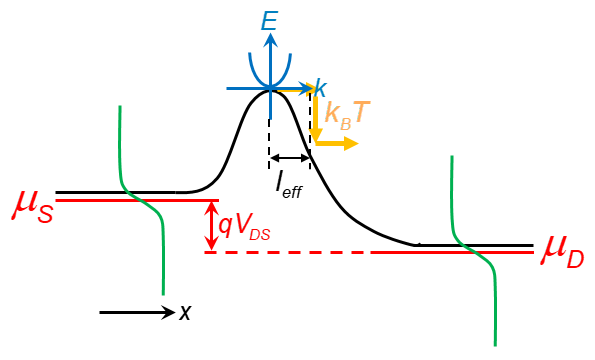
\includegraphics[width=0.6\textwidth]{figures/Fig5_1}
\centering
\caption{\small Band diagram of a small MOSFET.}
\end{figure}
In general, the current at the top-of-barrier can be expressed as \begin{equation}
    I = (-e)W(n_{S}^{+}v_{inj}^{+}-n_{S}^{-}v_{inj}^{-})
\end{equation} where the $n_{S}^{+(-)}$ are the numbers of electrons that injects to the $+x$- and $-x$-directions, the $v_{inj}^{+(-)}$ are the injection velocities to the $+x$- and $-x$-directions, and $W$ is the device width. The electron concentration $Q_{S}$ at the top-of-barrier is related to the gate voltage $V_{G}$. \begin{equation}
    Q_{S} = C(V_{G}-V_{REF})
\end{equation} where $C$ is the gate capacitance and $V_{REF}$ is the reference voltage that determines at which $V_{G}$ there is no electron in the channel. Since the Fermi level of drain side is far away from the conduction band edge in the channel, the electron injection from the drain can be neglected \begin{equation}
    I \approx (-e)Wn_{S}^{+}v_{inj}^{+}
\end{equation} and \begin{equation}
    n_{S} = n_{S}^{+} + n_{S}^{-} \approx n_{S}^{+} = \frac{C(V_{G}-V_{REF})}{-e}
\end{equation} Thus, \begin{equation}
    I = WC(V_{G}-V_{REF})v_{inj}^{+}
\end{equation} which describes the {\bf ballistic transport} in MOSFET.
\section{Transport with Scatterings (Quasi-Ballistic Transport)}
Since there are scatterings in the channel, there are some back-scattered electron $n_{S}^{-}$ but they are only small portion of the $+x$-direction injection \begin{equation}
    n_{S}^{-} = rn_{S}^{+}
\end{equation} where $r$ is the reflection coefficient. Note that the $n_{S}^{+(-)}$ are coming from the source side injection instead of the drain side as mentioned earlier. Since after scattering the electron only loses energy less or equal to $k_{B}T$, the back-scattered electron also has a velocity $v_{inj}^{-}$ close to the $v_{inj}^{+}$. Hence, the current becomes \begin{align}
    I& = (-e)Wn_{S}^{+}v_{inj}^{+}(1-r),\quad n_{S} = n_{S}^{+} + n_{S}^{-} = n_{S}^{+}(1+r)\nonumber\\
    & = (-e)n_{S}Wv_{inj}^{+}\frac{1-r}{1+r}W\nonumber\\
    & = WC(V_{G}-V_{REF})v_{inj}^{+}\frac{1-r}{1+r}
\end{align} Recall the transmission and reflection coefficients \begin{equation}
    T = \frac{\lambda}{\lambda + L}, \quad r = 1 - T = \frac{L}{\lambda + L}
\end{equation} The device length $L$ should be replaced by $l_{eff}$ as defined in Fig. 5.1 because the detailed simulations show that if the electron travels more than 1 to 2 times $\frac{k_{B}T}{q}$ down a potential drop, it is unlikely to re-emerge even if it does backscatter\footnote{M. Lundstrom, Fundamentals of Carrier Transport, 2nd edition, p. 344.}. Thus, the current becomes \begin{equation}
    I = WC(V_{G}-V_{REF})v_{inj}^{+}\frac{1}{1+2\frac{l_{eff}}{\lambda}}
\end{equation} Near equilibrium, the Einstein-Smoluchowski equation states that \begin{equation}
    \frac{2D}{\lambda} = v_{T},\quad \frac{D}{\mu} = \frac{k_{B}T}{e} 
\end{equation} where $D$ is the diffusion coefficient,$\mu$ is the low-field mobility, and $v_{T}$ is the thermal velocity. The electric field $E$ near the top-of-barrier can be estimated using \begin{equation}
    E_{top} = \frac{\frac{k_{B}T}{e}}{l_{eff}}\quad\Leftrightarrow\quad l_{eff} = \frac{k_{B}T}{eE_{top}}
\end{equation} Hence, \begin{align}
    I& = WC(V_{G}-V_{REF})v_{inj}^{+}\frac{1}{1+\frac{2k_{B}T/e}{\lambda E_{top}}},\quad \frac{2k_{B}T/e}{\lambda E_{top}}=\frac{2D}{\lambda}\frac{1}{\mu E_{top}} = \frac{v_{T}}{\mu E_{top}}\nonumber\\
    & = WC(V_{G}-V_{REF})\frac{v_{inj}^{+}}{1+\frac{v_{T}}{\mu E_{top}}}
\end{align} When the device is very long, $E_{top}$ is very small and thus $v_{T}\gg\mu E_{top}$. Thus, the current is back to the standard MOSFET current equation \begin{align}
    I& \approx W\mu C(V_{G}-V_{REF})\left(\frac{v_{inj}^{+}}{v_{T}}\right)E_{top}\nonumber\\
    & \approx \frac{W}{L}\mu C(V_{G}-V_{REF})\left(\frac{v_{inj}^{+}}{v_{T}}\right)V_{DS},\quad V_{DS} \approx \frac{E_{top}}{L}
\end{align}
\section{Generalized Ballistic Transport in One Dimension}
The concept of the injection velocity has been introduced in the previous sections. The injection velocity can be interpreted as the average velocity that the electrons travel from the top-of-the-barrier. \begin{equation}
    \big<v\big> = \frac{\sum_{k_{x}>0}{fv_{k_{x}}}}{\sum_{k_{x}>0}{f}}
\end{equation} where we define\footnote{The pre-factor is $\frac{1}{2\pi}$ instead of $\frac{L}{2\pi}$ because we are calculating the electron "density."} \begin{align}
    Z& \equiv \sum_{k_{x}>0}{fv_{k_{x}}} = \frac{1}{2\pi}\int_{0}^{\infty}dk_{x}\frac{1}{1+e^{\frac{E-\mu}{k_{B}T}}}\frac{\hbar k_{x}}{m^{*}},\quad E=E_{C}+\frac{\hbar^{2}k_{x}^{2}}{2m^{*}},\quad \frac{\mu-E_{C}}{k_{B}T}\equiv \eta \nonumber\\
    & = \frac{1}{2\pi}\frac{\hbar}{m^{*}}\int_{0}^{\infty}k_{x}dk_{x}\frac{1}{1+e^{\frac{\hbar^{2}k_{x}^{2}}{2m^{*}k_{B}T}}e^{-\eta}},\quad \frac{\hbar^{2}k_{x}^{2}}{2m^{*}k_{B}T}\equiv x\nonumber\\
    & = \frac{1}{2\pi}\frac{\hbar}{m^{*}}\frac{m^{*}k_{B}T}{\hbar^{2}}\int_{0}^{\infty}dx\frac{1}{1+e^{x-\eta}}\nonumber\\
    & = \frac{k_{B}T}{2\pi\hbar}\Gamma(1)\Im_{0}(\eta),\quad \Im_{p}(\eta) = \frac{1}{\Gamma(p+1)}\int_{0}^{\infty}dx\frac{x^{p}}{1+e^{x-\eta}}
\end{align} and \begin{align}
    Z_{2}& \equiv \sum_{k_{x}>0}{f} = \frac{1}{2\pi}\int_{0}^{\infty}dk_{x}\frac{1}{1+e^{\frac{\hbar^{2}k_{x}^{2}}{2m^{*}k_{B}T}}e^{-\eta}}\nonumber\\
    & = \frac{1}{2\pi}\frac{m^{*}k_{B}T}{\hbar^{2}}\frac{\hbar}{\sqrt{2m^{*}k_{B}T}}\int_{0}^{\infty}dx\frac{x^{-1/2}}{1+e^{x-\eta}}\nonumber\\
    & = \frac{1}{2\pi\hbar}\frac{\sqrt{m^{*}k_{B}T}}{\sqrt{2}}\sqrt{\pi}\Im_{-1/2}(\eta)
\end{align} Therefore, the average velocity is \begin{equation}
    \big<v\big> = \sqrt{\frac{2k_{B}T}{\pi m^{*}}}\frac{\Im_{0}(\eta)}{\Im_{-1/2}(\eta)}
\end{equation} where \begin{equation}
    \sqrt{\frac{2k_{B}T}{\pi m^{*}}} \equiv v_{T}
\end{equation} is the thermal velocity. If the semiconductor is non-degenerate doped ($\frac{E_{C}-\mu}{k_{B}T}\geq 3k_{B}T\Leftrightarrow \eta\geq -3$), the Fermi integral can be approximated by \begin{equation}
    \int_{0}^{\infty}dx\frac{1}{1+e^{x-\eta}}\approx\int_{0}^{\infty}dxe^{-x}e^{\eta} = e^{\eta}
\end{equation} Thus, \begin{equation}
    Z = \frac{k_{B}T}{2\pi\hbar}e^{\eta}
\end{equation} and \begin{equation}
    Z_{2} = \frac{\sqrt{m^{*}k_{B}T}}{2\pi\hbar}\frac{1}{\sqrt{2}}e^{\eta}\sqrt{\pi}
\end{equation} where \begin{equation}
    \int_{0}^{\infty}x^{-1/2}e^{-x} = \Gamma\left(\frac{1}{2}\right) = \sqrt{\pi}
\end{equation} For non-degenerate semiconductor, the average velocity is \begin{equation}
    \big<v\big> = \sqrt{\frac{2k_{B}T}{\pi m^{*}}} \approx 1.2\times10^7 \quad\text{cm/sec for silicon}
\end{equation} The ballistic current at the top-of-the barrier considering the injection from the source and drain is\footnote{In Section 5.1 and 5.2, the injection from the drain is ignored.} \begin{equation}
    I = W(-e)\underbrace{2}_{\text{spin}}\left(\sum_{k_{x}>0,k_{y}}{fv_{k_{x}}}-\sum_{k_{x}<0,k_{y}}{fv_{k_{x}}}\right)
\end{equation} where the first term is coming from the source side while the second term comes from the drain side \begin{align}
    F^{+}& \equiv \sum_{k_{x}>0,k_{y}}{fv_{k_{x}}} = \frac{1}{4\pi^{2}}\int_{-\infty}^{\infty}dk_{y}\int_{0}^{\infty}dk_{x}\frac{1}{1+e^{\frac{E-\mu_{S}}{k_{B}T}}}\frac{\hbar k_{x}}{m^{*}},\quad E=E_{C}+\frac{\hbar^{2}}{2m^{*}}\underbrace{\left(k_{x}^{2}+k_{y}^{2}\right)}_{k^{2}}\nonumber\\
    & = \frac{1}{4\pi^{2}}\int_{0}^{\pi}d\theta\int_{0}^{\infty}kdk\frac{1}{1+e^{\frac{\hbar^{2}k^{2}}{2m^{*}k_{B}T}}e^{-\eta_{S}}}\frac{\hbar}{m^{*}}k\sin{\theta}\nonumber\\
    & = \frac{1}{4\pi^{2}}\frac{\hbar}{m^{*}}2\frac{m^{*}k_{B}T}{\hbar^{2}}\frac{\sqrt{2m^{*}k_{B}T}}{\hbar}\underbrace{\int_{0}^{\infty}dx\frac{x^{1/2}}{1+e^{x-\eta_{S}}}}_{=e^{\eta_{S}}\Gamma(\frac{3}{2})\approx e^{\eta_{S}}\frac{\sqrt{\pi}}{2},\quad\text{if non-degenerate}}\nonumber\\
    & \approx \underbrace{\frac{1}{2}}_{\text{moving in $+x$ direction}}\underbrace{\left(\frac{m^{*}k_{B}T}{2\pi\hbar^{2}}\right)}_{\text{number of electrons within $k_{B}T$}}\underbrace{\left(\sqrt{\frac{2k_{B}T}{\pi m^{*}}}\right)}_{=v_{T}}e^{\eta_{S}}
\end{align} and \begin{equation}
    F^{-} \approx \frac{1}{2}\left(\frac{m^{*}k_{B}T}{2\pi\hbar^{2}}\right)\left(\sqrt{\frac{2k_{B}T}{\pi m^{*}}}\right)e^{\eta_{D}}
\end{equation} Therefore, the Equation (5.24) becomes \begin{align}
    I& = (-2e)W\frac{1}{2}\frac{m^{*}k_{B}T}{2\pi\hbar^{2}}v_{T}(e^{\eta_{S}}-e^{\eta_{D}})\nonumber\\
    & = (-e)W\frac{m^{*}k_{B}T}{2\pi\hbar^{2}}v_{T}e^{\eta_{S}}\left[1-e^{-(\eta_{S}-\eta_{D})}\right]\nonumber\\
    & = (-e)W\frac{m^{*}k_{B}T}{2\pi\hbar^{2}}v_{T}e^{\eta_{S}}\left[1-e^{-\frac{eV_{DS}}{k_{B}T}}\right]
\end{align} where \begin{equation}
    \eta_{S}-\eta_{D} = \frac{\mu_{S}-E_{C}}{k_{B}T}-\frac{\mu_{D}-E_{C}}{k_{B}T} = \frac{\mu_{S}-\mu_{D}}{k_{B}T} = \frac{eV_{DS}}{k_{B}T}
\end{equation} To link the Equation (5.27) to (5.1), we can calculate the charge density for $+x$ and $-x$ directions \begin{align}
    n_{S}^{+}& = \underbrace{2}_{\text{spin}}\sum_{k_{x}>0,k_{y}}{f} = 2\frac{1}{4\pi^{2}}\int_{0}^{\pi}d\theta\int_{0}^{\infty}kdk\frac{1}{1+e^{\frac{\hbar^{2}k^{2}}{2m^{*}k_{B}T}}e^{-\eta_{S}}}\nonumber\\
    & = 2\frac{1}{4\pi^{2}}\pi\frac{m^{*}k_{B}T}{\hbar^{2}}\int_{0}^{\infty}\frac{dx}{1+e^{x-\eta_{S}}} = \left(\frac{m^{*}k_{B}T}{2\pi\hbar^{2}}\right)e^{\eta_{S}}
\end{align} and \begin{equation}
    n_{S}^{-} = 2\sum_{k_{x}<0,k_{y}}{f} = \left(\frac{m^{*}k_{B}T}{2\pi\hbar^{2}}\right)e^{\eta_{D}}
\end{equation} The totla charge density $n_{S}$ is \begin{equation}
    n_{S} = n_{S}^{+} + n_{S}^{-} = \left(\frac{m^{*}k_{B}T}{2\pi\hbar^{2}}\right)\left(e^{\eta_{S}}+e^{\eta_{D}}\right) = \left(\frac{m^{*}k_{B}T}{2\pi\hbar^{2}}\right)e^{\eta_{S}}\left(1+e^{-\frac{eV_{DS}}{k_{B}T}}\right)
\end{equation} Therefore, the Equation (5.27) becomes \begin{align}
    I& = \underbrace{(-e)n_{S}}_{\equiv Q_{S}=C(V_{G}-V_{REF})}Wv_{T}\left(\frac{1-e^{-\frac{eV_{DS}}{k_{B}T}}}{1+e^{-\frac{eV_{DS}}{k_{B}T}}}\right)\nonumber\\
    & = WC(V_{G}-V_{REF})\underbrace{v_{T}\left(\frac{1-e^{-\frac{eV_{DS}}{k_{B}T}}}{1+e^{-\frac{eV_{DS}}{k_{B}T}}}\right)}_{\equiv v_{inj}}
\end{align} As increasing $V_{DS}$, the injection velocity $v_{inj}$ gradually approaches to the thermal velocity $v_{T}$ which is similar to the velocity saturation concept in the traditional semiconductor device textbook. When $V_{DS} < \frac{k_{B}T}{e}$, $e^{-\frac{eV_{DS}}{k_{B}T}}\approx 1-\frac{eV_{DS}}{k_{B}T}$. Thus, the Equation (5.32) becomes \begin{align}
    I& \approx WC(V_{G}-V_{REF})v_{T}\frac{V_{DS}}{2k_{B}T/e}\nonumber\\
    & = \frac{W}{L}C(V_{G}-V_{REF})\underbrace{\left(\frac{Lv_{T}}{2k_{B}T/e}\right)}_{\mu_{B}}V_{DS}
\end{align} where $\mu_{B}$ is the ballistic mobility\footnote{M. S. Shur, "Low Ballistic Mobility in Submicron HEMTs," IEEE Electron Device Letter, vol. 23, no. 9, pp. 511-513, Sept. 2002.} since \begin{equation}
    v_{T} = \sqrt{\frac{2k_{B}T}{\pi m^{*}}} \Rightarrow 2k_{B}T = v_{T}^{2}\pi m^{*}
\end{equation} \begin{equation}
    \Rightarrow \frac{Lv_{T}}{2k_{B}T/e} = \frac{e}{m^{*}}\underbrace{\frac{L}{\pi v_{T}}}_{\tau} \equiv \frac{e}{m^{*}}\tau \equiv \mu_{B}
\end{equation} It is observed that the ballistic mobility is a linear function of $L$. As shortening $L$, the ballistic mobility decreases which is different from the prediction of scatterings in the channel. In other words, when $L$ is large enough, the mobility should decrease with longer length since there are more scattering. Therefore, this linear relation provides us the insight of the ballistic transport happening.
\section{Generalized Quasi-Ballistic Transport}
In previous section, we've derived the ballistic current model. Now, let's consider the reflection in the injection from both source and drain, i.e., quasi-ballistic current model. The electron density at the top-of-the-barrier is \begin{equation}
    n_{S} = n_{S}^{+}(1-r_{S}) + n_{S}^{-}(1-r_{D}) + r_{S}n_{S}^{+} = n_{S}^{+} + n_{S}^{-}(1-r_{D})
\end{equation} where $r_{S,D}$ are the reflection coefficients from the source and drain. Furthermore, the quasi-ballistic current can expressed as \begin{align}
    I& = 2(-e)W\left[\sum_{k_{x}>0,k_{y}}{fv_{k_{x}}(1-r_{S})}-\sum_{k_{x}<0,k_{y}}{fv_{k_{x}}(1-r_{D})}\right]\nonumber\\
    & = 2(-e)W\left[(1-r_{S})\sum_{k_{x}>0,k_{y}}{fv_{k_{x}}}-(1-r_{D})\sum_{k_{x}<0,k_{y}}{fv_{k_{x}}}\right]\nonumber\\
    & = (-e)W\frac{m^{*}k_{B}T}{2\pi\hbar^{2}}v_{T}e^{\eta_{S}}\left[(1-r_{S})-(1-r_{D})e^{-\frac{eV_{DS}}{k_{B}T}}\right]\nonumber\\
    & = WC(V_{G}-V_{REF})v_{T}\left[\frac{(1-r_{S})-(1-r_{D})e^{-\frac{eV_{DS}}{k_{B}T}}}{1+(1-r_{D})e^{-\frac{eV_{DS}}{k_{B}T}}}\right]\nonumber\\
    & = WC(V_{G}-V_{REF})v_{T}\frac{1-r_{S}}{1+r_{S}}\frac{1-\frac{1-r_{D}}{1-r_{S}}e^{-\frac{eV_{DS}}{k_{B}T}}}{\frac{1}{1+r_{S}}+\frac{1-r_{D}}{1+r_{S}}e^{-\frac{eV_{DS}}{k_{B}T}}}
\end{align} where \begin{equation}
    n_{S} = \left(\frac{m^{*}k_{B}T}{2\pi\hbar^{2}}\right)e^{\eta_{S}}\left[]1+(1-r_{D})e^{-\frac{eV_{DS}}{k_{B}T}}\right] = C(V_{G}-V_{REF})
\end{equation} Recall the Equation (5.8) and (5.9), the Equation (5.37) becomes \begin{equation}
    I =  WC(V_{G}-V_{REF})\frac{v_{T}}{1+\frac{2l_{eff}}{\lambda}}\frac{1-\frac{1-r_{D}}{1-r_{S}}e^{-\frac{eV_{DS}}{k_{B}T}}}{\frac{1}{1+r_{S}}+\frac{1-r_{D}}{1+r_{S}}e^{-\frac{eV_{DS}}{k_{B}T}}}
\end{equation} Normally $r_{S,D}$ are close to zero since the electrons are not localized. In practical model fitting, $r_{S,D}$ are often the model parameters for fitting.
\section{Anisotropic Effective Mass in Ballistic Transport}
In previous section, the isotropic effective mass is assumed, i.e., $m_{x} = m_{y} = m^{*}$. Now, if $m_{x}\neq m_{y}$, the charge density ($n_{S}$) and electron flux ($F$) should be re-written by modifying the Fermi function. \begin{equation}
    f = \frac{1}{1+e^{\frac{E-\mu_{S,D}}{k_{B}T}}} = \frac{1}{1+e^{\left(\frac{\hbar^{2}k_{x}^{2}}{2m_{x}}+\frac{\hbar^{2}k_{y}^{2}}{2m_{y}}\right)/k_{B}T}e^{\frac{-(\mu_{S,D}-E_{C})}{k_{B}T}}}
\end{equation} If defining \begin{equation}
    k_{x}' = \frac{k_{x}}{\sqrt{m_{x}}},\quad k_{y}' = \frac{k_{y}}{\sqrt{m_{y}}}, \quad k'^{2} = k_{x}'^{2}+k_{y}'^{2}
\end{equation} the similar integrations to the Equation (5.25), (5.26), (5.29), and (5.30), can be made assuming non-degenerated doping and give \begin{equation}
    n_{S} = \frac{\sqrt{m_{x}m_{y}}k_{B}T}{2\pi\hbar^{2}}e^{\eta_{S}}\left(1+e^{-\frac{eV_{DS}}{k_{B}T}}\right)
\end{equation} and \begin{equation}
    F^{+,-} = \frac{1}{2}\frac{\sqrt{m_{x}m_{y}}k_{B}T}{2\pi\hbar^{2}}\sqrt{\frac{2k_{B}T}{\pi m_{x}}}e^{\eta_{S,D}}
\end{equation} Therefore, the ballistic current considering the anisotropic effective mass is \begin{equation}
    I = (-e)W\frac{\sqrt{m_{x}m_{y}}k_{B}T}{2\pi\hbar^{2}}\sqrt{\frac{2k_{B}T}{\pi m_{x}}}e^{\eta_{S}}\left(1-e^{-\frac{eV_{DS}}{k_{B}T}}\right)
\end{equation} Notice that the current only depends on the effective mass in the direction perpendicular to the transport, which determines the electron density. Although the silicon has a high DOS close to metal, the gate dielectric cannot support such high electric field that achieves the high electron density. Now, if there are multiple subbands (assume $z$-direction is confined while $x$ and $y$ are not, i.e., two-dimensional electron gas), the total current is \begin{equation}
    I = \sum_{n=1}^{N}{(-e)W\frac{\sqrt{m_{x}m_{y}}k_{B}T}{2\pi\hbar^{2}}\sqrt{\frac{2k_{B}T}{\pi m_{x}}}e^{\frac{\mu_{S}-E_{C}^{n}}{k_{B}T}}\left(1-e^{-\frac{eV_{DS}}{k_{B}T}}\right)}
\end{equation} where \begin{equation}
    E_{C}^{n} = E_{C0} + \frac{\hbar^{2}n^{2}\pi^{2}}{2m_{z}L_{z}^{2}} + \frac{\hbar^{2}k_{x}^{2}}{2m_{x}} + \frac{\hbar^{2}k_{y}^{2}}{2m_{y}}
\end{equation} is the band edge of the $n$th subband, $N$ is the total number of subbands, and $L_{z}$ is the $z$-direction thickness. Note that the band-to-band scattering is ignored here to simplify the problem.
\section{Issues of Scaling MOSFETs}
\subsubsection{Degraded Threshold Voltage and Subthreshold Slope\protect\footnote{This lecture was taught by Prof. Jeffery Bokor. The topics of this section have been covered by EE230B. One may refer to: Y. Taur and T. H. Ning, Fundamentals of Modern VLSI Devices, 2nd edition, 2009.}}
In short channel MOSFETs, the electrostatic control from the drain becomes comparable to the gate control as shown in Fig. 5.2.
\begin{figure}[tbp]
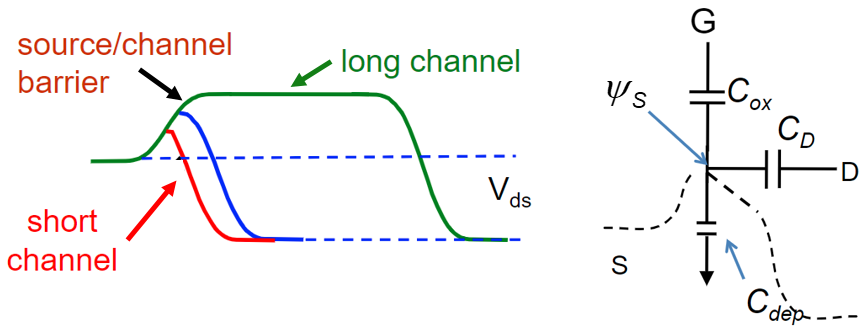
\includegraphics[width=0.8\textwidth]{figures/Fig5_2}
\centering
\caption{\small Illustration of channel potentials with various gate lengths and the equivalent circuit.}
\end{figure}
Similar to the concept in Chapter 1, the potential at the top-of-the-barrier can be written as \begin{equation}
    \psi_{S} = \frac{C_{OX}}{C_{OX}+C_{dep}+C_{D}}V_{GS} + \frac{C_{D}}{C_{OX}+C_{dep}+C_{D}}V_{DS}
\end{equation} where $C_{dep}$ is the depletion capacitance of the channel. From the Equation (5.47), $C_{D}$ gradually increase with shortening the gate length, and thus the drain voltage starts to control the barrier. If $V_{DS}$ is high, the threshould voltage ($V_{TH}$) is significantly degraded. This is called the {\bf drain-induced barrier lowering (DIBL)}. Furthermore, since the channel potential (charges) is controlled by (shared with) the drain terminal (even the source terminal), the threshold voltage is also decreasing even when $V_{DS}$ is low, which is known as {\bf $V_{TH}$ roll off}. The additional control from the drain terminal also deteriorates the subthreshold slope $SS$ \begin{equation}
    SS \equiv \left[\frac{\partial \log{I_{DS}}}{\partial V_{GS}}\right]^{-1} = 60\text{[mV/dec]}\times\left(1+\frac{C_{dep}+C_{D}}{C_{OX}}\right)
\end{equation} This is undesired since it significantly increases the OFF-state leakage current.
\subsubsection{Gate Tunneling Leakage}
Since the gate length is scaled to boost the current and allow more transistors in a give chip area, the gate oxide should be also scaled to improve the gate control as shown in the Equation (5.47). However, the thin oxide could lead to significant gate leakage due to the direct tunneling. Therefore, the high-$\kappa$ dielectric was introduced in the 45-nm technology node to keep the gate capacitance but increase the physical oxide thickness. Nevertheless, there are still some difficulties of the high-$\kappa$ dielectric: (1) chemical reactions between them and the silicon substrate and gate; (2) lower surface mobility than the Si/SiO$_{2}$ system; (3) too low a $V_{TH}$ for P-channel MOSFET (as if there is positive charge in the high-$\kappa$ dielectric); (4) long-term reliability; (5) a thin SiO$_{2}$ interfacial layer may be inserted between Si-substrate and high-$\kappa$ film.
\subsubsection{Mitigating Short Channel Effect of MOSFET}
Since the channel potential is also controlled by $C_{dep}$ and $C_{D}$, decreasing the depletion width by increasing the body doping is helpful but it may reduce the mobility due to the impurity scattering. Furthermore, using high-$\kappa$ metal gate as mentioned earlier also overcomes the poly-depletion problem. To cut the leakage path underneath the channel due to lack of gate control, the shallow junction is adopted. However, it enlarges the series resistance and thus degrades the ON-state current. To improve the mobility, strained silicon is used in the channel. In addition to the mentioned techniques to improve the device performances of the traditional MOSFET, new transistor structures [e.g. fully-depleted SOI (FDSOI) and FinFET] and new device operation mechanisms [e.g. tunnel FET (TFET) and negative capacitance FET (NCFET)] are proposed. The FDSOI can cut the leakage path and achieve low leakage, and the FinFET improves the gate control by increasing the gate capacitance. Furthermore, the TFET utilizes the tunneling mechanism which overcomes the problem from Boltzmann distribution, and the NCFET can achieve better subthreshold behavior since the channel potential can be boosted by the ferrroelctric layer sandwiched by the metal gate and interfacial layer.
\section{Application of the Developed Current Model}
The ballistic and quasi-ballistic current models have been derived. In this section, how the developed model relates to the real measurement data will be examined. Recall the Equation (5.47). At low $V_{GS}$ (let's say OFF-state), if the FDSOI or FinFET structure is adopted, the surface potential ($\psi_{S}$) in the channel is \begin{equation}
    \psi_{S} = \frac{C_{OX}}{C_{OX}+C_{D}}V_{GS} + \frac{C_{D}}{C_{OX}+C_{D}}V_{DS} \equiv \alpha_{G}V_{GS} + \alpha_{D}V_{DS}
\end{equation} where the contribution from the charge $Q$ is relatively small. The quasi-ballistic current is \begin{align}
    I^{OFF}& = (-e)W\frac{\sqrt{m_{x}m_{y}}k_{B}T}{2\pi\hbar^{2}}\sqrt{\frac{2k_{B}T}{\pi m_{x}}}e^{\frac{\mu_{S}}{k_{B}T}}e^{-\frac{E_{C}}{k_{B}T}}\left(1-e^{-\frac{eV_{DS}}{k_{B}T}}\right)/\left(1+\frac{2l_{eff}}{\lambda}\right),-E_{C}\rightarrow e\psi_{S}\nonumber\\
    & = (-e)W\frac{\sqrt{m_{x}m_{y}}k_{B}T}{2\pi\hbar^{2}}\sqrt{\frac{2k_{B}T}{\pi m_{x}}}e^{\frac{\mu_{S}}{k_{B}T}}e^{\frac{e\psi_{S}}{k_{B}T}}\left(1-e^{-\frac{eV_{DS}}{k_{B}T}}\right)/\left(1+\frac{2l_{eff}}{\lambda}\right)\nonumber\\
    & = Ae^{\frac{\alpha_{G}V_{GS}}{k_{B}T/e}}e^{\frac{\alpha_{D}V_{DS}}{k_{B}T/e}}\left(1-e^{-\frac{eV_{DS}}{k_{B}T}}\right) = Be^{\frac{\alpha_{G}V_{GS}}{k_{B}T/e}}
\end{align} Thus, the subthreshold slope is \begin{align}
    SS& = \left[\frac{\partial \log{I}}{\partial V_{GS}}\right]^{-1} = \frac{2.3k_{B}T/e}{\alpha} = 60/\alpha_{G}\text{[mV/dec]}\nonumber\\
    &= 60\times\left(1+\frac{C_{D}}{C_{OX}}\right)\text{[mV/dec]}\equiv 60\times m\text{[mV/dec]}
\end{align} where $m$ is called the body factor. The DIBL is defined as \begin{equation}
    \text{DIBL} = \frac{V_{TH}^{low}-V_{TH}^{high}}{V_{DS}^{high}-V_{DS}^{low}}\quad\text{[mV/V]}
\end{equation} where the threshold voltage $V_{TH}$ is defined using the constant current method \begin{equation}
    I_{TH} = Ae^{\frac{e\psi_{S}^{high}}{k_{B}T}} = Ae^{\frac{e\psi_{S}^{low}}{k_{B}T}}\frac{V_{DS}}{k_{B}T/e}
\end{equation} since \begin{equation}
    \left(1-e^{-\frac{eV_{DS}}{k_{B}T}}\right)\approx \frac{eV_{DS}}{k_{B}T},\quad\text{at low $V_{DS}$}\nonumber
\end{equation} where "low" and "high" denote as low and high $V_{DS}$, and \begin{equation}
    \psi_{S}^{low} = \alpha_{G}V_{TH}^{low} + \alpha_{D}V_{DS}^{low}
\end{equation} and \begin{equation}
    \psi_{S}^{high} = \alpha_{G}V_{TH}^{high} + \alpha_{D}V_{DS}^{high}
\end{equation} Thus, \begin{equation}
    \text{DIBL} = \frac{\alpha_{D}}{\alpha_{G}}-\frac{1}{\alpha_{G}}\frac{\psi_{S}^{high}-\psi_{S}^{low}}{V_{DS}^{high}-V_{DS}^{low}}
\end{equation} However, from the Equation (5.53) we have \begin{equation}
    \psi_{S}^{high}-\psi_{S}^{low} = \frac{k_{B}T}{e}\left[\ln{\frac{I_{TH}}{A}}-\ln{\frac{I_{TH}}{A}\frac{V_{DS}^{low}}{k_{B}T/e}}\right] = \frac{k_{B}T}{e}\ln{\frac{V_{DS}^{low}}{k_{B}T/e}}
\end{equation} which is very small since $V_{DS}^{low}$ is 50 mV\footnote{$V_{DS} =$ 50 mV is called the linear $V_{DS}$ and is commonly used. If applying $V_{DS} = $ 26 mV, the thermal noise could be an issue.}. Therefore, \begin{equation}
    \text{DIBL} = \frac{\alpha_{D}}{\alpha_{G}} = \frac{C_{D}}{C_{OX}}
\end{equation} which can be extracted from the subthreshold slope or the body factor.

\end{document}